\documentclass[12pt]{book}

% ------------------------------------------------------------
% PACCHETTI BASE
% ------------------------------------------------------------
\usepackage[utf8]{inputenc}    % Accenti
\usepackage[T1]{fontenc}       % Font moderni
\usepackage[italian]{babel}    % Lingua italiana
\usepackage{graphicx}          % Immagini
\usepackage{geometry}          % Margini
\usepackage{float}             % [H] per posizionare le figure
\usepackage{hyperref}          % Link cliccabili
\usepackage[normalem]{ulem}    % Sottolineature
\usepackage{soul}              % Evidenziare testo
\usepackage{xcolor}            % Colori
\usepackage{amsmath}           % Matematica
\usepackage{caption}           % Gestione didascalie
\usepackage{placeins}          % \FloatBarrier
\usepackage{titlesec}          % Controllo spazi titoli
% \usepackage{lipsum}          % Solo per testo fittizio
% ------------------------------------------------------------


% ------------------------------------------------------------
% STRUTTURA SEZIONI E NUMERAZIONE
% ------------------------------------------------------------
\setcounter{secnumdepth}{4}
\setcounter{tocdepth}{4}
% ------------------------------------------------------------


% ------------------------------------------------------------
% GEOMETRIA PAGINA
% ------------------------------------------------------------
\geometry{
  a4paper,
  left=2cm,
  right=2cm,
  top=2cm,
  bottom=2cm
}
% ------------------------------------------------------------


% ------------------------------------------------------------
% SPAZIATURA GENERALE
% ------------------------------------------------------------
\setlength{\parskip}{3pt plus 1pt minus 1pt}  % Spazio tra paragrafi
\setlength{\parindent}{15pt}                  % Rientro dei paragrafi

% Spazi figure e didascalie
\setlength{\textfloatsep}{8pt plus 2pt minus 2pt}
\setlength{\intextsep}{8pt plus 2pt minus 2pt}
\setlength{\abovecaptionskip}{4pt plus 1pt minus 1pt}
\setlength{\belowcaptionskip}{4pt plus 1pt minus 1pt}

% Compatta titoli e sottosezioni
\titlespacing*{\section}{0pt}{10pt plus 2pt minus 2pt}{6pt plus 1pt minus 1pt}
\titlespacing*{\subsection}{0pt}{8pt plus 1pt minus 1pt}{4pt plus 1pt minus 1pt}
\titlespacing*{\subsubsection}{0pt}{6pt plus 1pt minus 1pt}{3pt plus 1pt minus 1pt}
% ------------------------------------------------------------


% ------------------------------------------------------------
% PREVENZIONE FIGURE ISOLATE / PAGINE VUOTE
% ------------------------------------------------------------
\widowpenalty=10000     % Evita righe singole in fondo pagina
\clubpenalty=10000      % Evita righe singole in cima
\brokenpenalty=10000    % Evita interruzioni di riga brutte
\raggedbottom            % Impedisce di “stirare” verticalmente il testo

% Figure e tabelle: mantieni almeno metà pagina di testo
\renewcommand{\floatpagefraction}{.7}   % Una figura occupa max 70% della pagina
\renewcommand{\textfraction}{.2}        % Almeno 20% di testo nella pagina
\renewcommand{\topfraction}{.9}         % Figure in cima: fino al 90%
\renewcommand{\bottomfraction}{.8}      % Figure in basso: fino all’80%
% ------------------------------------------------------------


% ------------------------------------------------------------
% DATI DOCUMENTO
% ------------------------------------------------------------
\title{Informatica Giuridica}
\author{Antonio Runcio}
\date{Aprile 2025}
% ------------------------------------------------------------


\includeonly{40_cap_4} % Compila solo il capitolo specificato
% ------------------------------------------------------------


\begin{document}

\frontmatter
% \tableofcontents % Indice (se serve)

\mainmatter
\pagestyle{plain} % Numeri di pagina in basso al centro


% ------------------------------------------------------------
% CAPITOLI
% ------------------------------------------------------------
\chapter{Lezione 1 - Approccio quantitativo al progetto e all'analisi. Parte 1}


In questo corso ci occuperemo dell'architettura dei sistemi di elaborazione, della loro descrizione sia interna che funzionale. Inizieremo questo ciclo di lezioni affrontando e descrivendo un approccio quantitativo al progetto e all'analisi. Questa lezione è costituita da due parti, oggi ci occuperemo della prima parte.
Ogni lezione sarà organizzata descrivendovi un sommario in cui affronteremo i problemi della lezione. Il primo argomento del sommario sono le tendenze nell'industria dei calcolatori. Successivamente discuteremo brevemente dell'era post PC


Argomenti trattati:
\begin{itemize}
    \item tendenze nell'industria dei calcolatori
    \item L'era Post-PC
\end{itemize}

Cominciamo con affrontare il primo degli argomenti, le tendenze nell'industria dei calcolatori.

\section{Tendenze nell'industria dei calcolatori}

Quando intendo dire tendenze, intendo dire l'evoluzione storica che sia avuta negli anni.

Durante la seconda guerra mondiale i calcolatori elettromeccanici ed elettronici per la decriptazione di codici furono sviluppati prevalentemente dai britannici e dagli americani per decriptare il cosiddetto Enigma, che era un sistema di decriptazione utilizzato per consentire le comunicazioni da e per i sottomarini tedeschi che affondavano ripetutamente le navi che transitavano attraverso l'Atlantico, trasportando materiali e uomini dagli Stati Uniti alla Gran Bretagna durante le prime fasi della guerra.

Questo è stato chiaramente un argomento di evidente rilevanza per il momento che ha portato le migliori menti a cimentarsi per la prima volta nell'utilizzo di macchine automatiche finalizzate a rompere questi codici, cioè a capire quali fossero le chiavi dei codici e quindi una volta identificate le chiavi poter decriptare i messaggi trasmessi. Ovviamente quando l'algoritmo fu decriptato non fu fatto scoprire ai tedeschi anche con non poco sacrificio delle proprie forze umane.
La cosa però è importante capire è che c'è stato un fortissimo motore che ha spinto lo sviluppo della tecnologia.
Notate che nella slide fig. \ref{fig:slide_4} è scritto esplicitamente calcolatori elettromeccanici ed elettronici.

\begin{figure}[ht]
    \centering
    \includegraphics[width=0.6\linewidth]{images/Lez01_P01_fig_04.png}
    \caption{Slide 4}
    \label{fig:slide_4}
\end{figure}

Con questo intendo dire che i calcolatori, per come la maggior parte di voi ormai è familiare, sono ben lontani da quello che erano agli albori dello sviluppo.
Il termine di elettromeccanici si intende che i selettori commutatori erano fisicamente degli oggetti meccanici, non molto dissimili dalle centrali di comunicazione telefoniche, in cui vi sono delle levette che venivano un azionate attraverso sistemi elettromeccanici tipo dei solenoidi, anche se già negli stessi anni, durante i primi anni 40, si andavano affermando i primi sistemi elettronici basati su tubi a vuoto, cioè delle valvole.

Nel breve si sviluppò anche il cosiddetto Electronic Numerical Integrator and Calculator, detto anche ENIAC, che fu il primo calcolatore elettronico d'uso generale, sviluppato anche esso durante la seconda guerra mondiale, ma reso pubblico soltanto nel 1947.
Notate la differenza fra la prima riga e la seconda riga?

Nella prima riga si parla di sistemi dedicati per la decriptazione di codici, quindi che sia elettromeccanici o elettronici non è particolarmente rilevante in questa fase, l'importante è osservare che i primi sistemi erano specificamente dedicati a un solo compito.
Nella seconda riga, quando parliamo di calcolatore d'uso generale, intendiamo un calcolatore che possa svolgere in linea di principio qualunque programma.
Il nome dice sostanzialmente che è un sistema per calcolare e integrare numericamente, quindi è elettronico.
Questo è definito un sistema ad uso generale perché può in linea di principio calcolare qualunque operazione e integrare in realtà qualunque funzione.
La cosa curiosa, forse quasi pittoresca, è che ENIAC aveva 18.000 tubi a vuoto come elementi logici.
18.000 tubi a vuoto ovviamente per gli anni determinavano una struttura esageratamente ingombrante, sia in termini di spazio che di potenza dissipata.
Queste erano strutture della dimensione equivalente di una lampadina e quindi ovviamente occupavano molto spazio.
La potenzialità di calcolo di ENIAC era comunque oggettivamente esigua.
Eseguiva una ADD, cioè un'operazione di addizione in 200 microsecondi, sostanzialmente 5000 istruzioni al secondo.
Se andiamo a paragonarla ai tempi attuali, ovviamente erano dei numeri veramente modesti, ma consentivano questi calcolatori ENIAC in particolare di calcolare tabelle di tiro per consentire quindi in particolare ai cannoni navali antiaereo di andare a colpire aerei in movimento.
Ovviamente considerate che vi sono diverse componenti da tenere in conto, quindi la gravità, l'attrito dell'aria, le traiettorie sia dei proiettili che degli aeroplani e questo ovviamente fatto a mano non era ovviamente agevole, quindi era necessario calcolare delle tabelle di tiro che poi date agli operatori, consentivano a loro con delle più semplici misurazioni di poter colpire il bersaglio.

Mi dispiace parlare di queste cose, ma questo è stato determinante dal punto di vista dello sviluppo.
Se non ci fosse stata quella necessità probabilmente voi oggi non avreste il vostro iPad, il vostro iPhone o Android o quello che sia.
Il punto di avvio della tecnologia è stato in questo caso a noi determinato da interessi di natura militare per la sopravvivenza degli Stati.

\begin{figure}[ht]
    \centering
    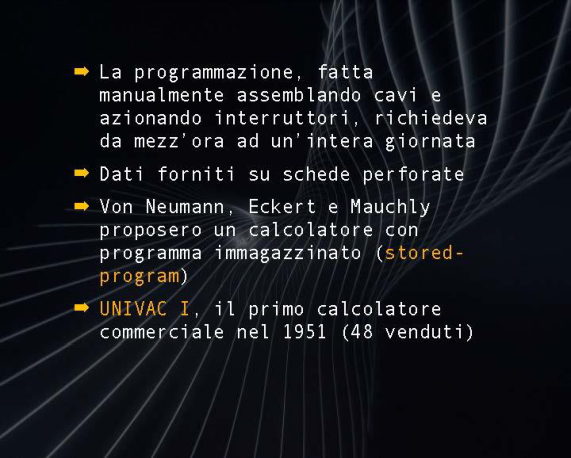
\includegraphics[width=0.6\linewidth]{images/Lez01_p01_fig_05.png}
    \caption{Slide 5}
    \label{fig:slide_5}
\end{figure}

La programmazione  di Enec (slide \ref{fig:slide_5}) veniva fatta manualmente assemblando cavi e azionando interruttori e richiedeva tipicamente da mezz'ora a un'intera giornata.
Notate la frase assemblando, la parola assemblatore deriva esattamente dalla funzione degli operatori che andavano fisicamente ad assemblare cavi, muovere interruttori, aggiungere schede e parti per riprogrammare questo calcolatore.
Quindi non vi era un programma immagazzinato su un supporto di massa, un disco, una memoria stato solido, un nastro o qualunque altro mezzo di archiviazione, ma il programma veniva scritto fisicamente ogni volta ricablando e riposizionando degli interruttori.
Ovviamente era una cosa esageratamente primitiva dal nostro punto di vista ma è importante osservare anche alcune delle ragioni storiche che determinano l'uso di certi terminologie, in particolare del termine assemblatore.
I dati in uscita venivano forniti su schede perforate che era un sistema di rappresentazione dell'informazione in uscita abbastanza semplice ma comunque già gestibile dagli utenti in maniera ragionevolmente semplice.

In quegli anni anche Von Neumann, Eckhart e Mauclky proposero un calcolatore con un programma immagazzinato, quello che in inglese si chiama store program.
In questo caso per cambiare il programma non è più necessario ricablare il sistema, bensì è possibile caricarlo in qualche modo da qualche altra forma di supporto.
Questo è il concetto generale di tutti i programmi che noi ogni giorno utilizziamo, nessuno di noi penserebbe mai di dover ricablare il proprio calcolatore per poter svolgere una nuova funzione.

Di lì a poco Univac 1 fu il primo calcolatore commerciale ed entrò in commercio nel 1951, ben 48 pezzi furono venduti.
Anche questa è una macchina oggettivamente molto ingombrante, molto grande.
Di lì a poco seguì anche l'IBM, che era un'azienda che si occupava di sistemi di stampa, archivi e ufficio, quindi avevano chiaramente un mercato diretto da aggredire.
Questi piccoli cenni storici vi li do anche perché è importante contestualizzare le evoluzioni.

\begin{figure}[ht]
    \centering
    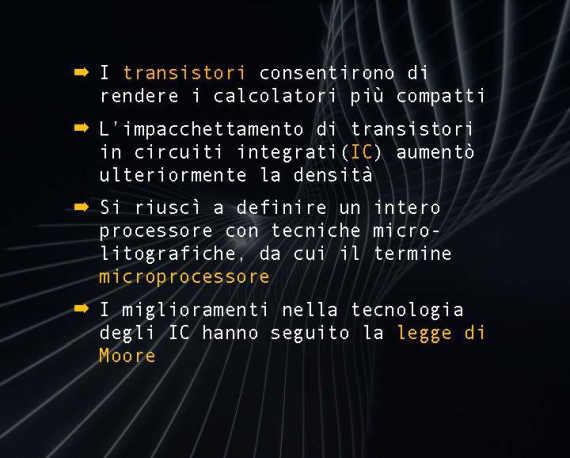
\includegraphics[width=0.6\linewidth]{images/Lez01_p01_fig_06.png}
    \caption{Slide 6}
    \label{fig:slide_6}
\end{figure}

I transistori (slide \ref{fig:slide_6}) a stato solido consentirono di rendere i calcolatori ben più compatti di quanto non erano mediante l'utilizzo di valvole a vuoto.
Col tempo si riuscirono a impacchettare transistori in circuiti integrati o integrated circuits in inglese e ciò aumentò ulteriormente la densità dei transistori per unità di superficie.
Questo è particolarmente importante, per poter fare cose più evolute e più potenti spesso è necessario avere più dispositivi.
Ricordate quello che vi ho detto in una delle precedenti slide, ENIAC aveva 18.000 valvole.
Se andate a stimare nell'ordine di qualche centimetro cubo il volume di una valvola fate presto a fare i conti di quanto è ingombrante il sistema.
Oggigiorno un transistore ha delle dimensioni fra i 20 e i 14 nanometri, come di dimensione del disegno.
Ovviamente è una struttura prevalentemente bidimensionale e quindi il volume reale dei dispositivi di commutazione è veramente esiguo, quello che vincola prevalentemente è la superficie e non tanto il volume in questo caso.

Col passare del tempo e dello sviluppo tecnologico si riuscì a definire un intero processore con tecniche microlitografiche da cui ha anche il termine di microprocessore, cioè si riuscirono a mettere tutti i transistori in un solo chip, cioè una lastrina di silicio, in modo tale da poter svolgere tutte le funzioni.
Il primo microprocessore propiamente detto fu sviluppato nel 1971 e fu utilizzato dalla Texas Instruments per una piccolissima calcolatrice, tipicamente quella con cui voi normalmente fate somme e sottrazioni o poco più.
Ovviamente doveva essere un sistema a bassissimo costo, doveva essere venduto in un oggetto veramente consumer, cioè di largo utilizzo e ovviamente non particolarmente dedicato.

Quindi i primi microprocessori furono veramente delle macchine minimaliste, spesso a 4 bit, sia quello della Texas Instruments, il TMS 1000, che di lì a pochissimi mesi il 4004 dell'Intel, che fu un antisignano di una lunghissima generazione di processori che di fatto determinano che questa azienda in buona parte domini una parte del mercato, non tutti i mercati, ma una parte dei mercati.

I miglioramenti della tecnologia dei circuiti integrati hanno seguito la cosiddetta legge di Moore.

Nel caso voi non abbiate già avuto occasione di leggere o sentirla nella definizione corretta, ve la do nella slide \ref{fig:slide_7}.

\begin{figure}[ht]
    \centering
    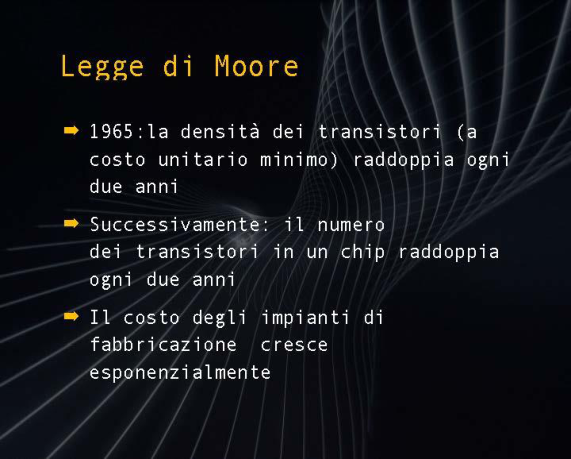
\includegraphics[width=0.6\linewidth]{images/Lez01_p02_fig_01.png}
    \caption{Slide 7}
    \label{fig:slide_7}
\end{figure}

La versione formulata nel 1965 da Gordon Moore, uno dei fondatori della Intel: \textit{"La densità dei transistori a costo unitario minimo raddoppia ogni due anni".}

%11:56
Questa osservazione fu fatta da una semplice osservazione sperimentale dell'andamento degli ultimi anni, da quando si era cominciato a integrare un numero di transistori crescente sullo stesso chip di silicio.
Quello che osservò Gordon Moore fu che era possibile ogni due anni raddoppiare il numero dei transistori mantenendo il minimo prezzo per transistori.
Da questa formulazione ne derivò una formulazione differente, quasi un corollario, che successivamente si disse che il numero dei transistori in un chip raddoppia ogni due anni.
Notate le due formulazioni sembrano identiche ma in realtà non lo sono.
Quello che è importante osservare non è che a prescindere da tutto il numero dei transistori raddoppi ogni anno, quello che succede è che è possibile realizzare transistori a costo minimo con un costo che permette l'aumento della densità di un fattore 2.
Sfortunatamente a questa crescita esponenziale del numero dei transistori per unità di superficie è anche derivato che il costo degli impianti di fabbricazione cresce esponenzialmente.
Quindi l'industria vive solo se è in grado di produrre sempre più transistori per mantenere lo stesso volume di mercato.
Ovviamente poi aggredisce anche nuovi mercati e questo fa sì che gli investimenti possono crescere e quindi gli sviluppi andino più oltre.
Le ultime due righe ci dicono che sostanzialmente per molti anni voi avete pagato la stessa cifra per avere delle performance che in buona sostanza in prima approssimazione raddoppiavano.
I miglioramenti nei linguaggi di programmazione ad alto livello inoltre hanno reso sostanzialmente desueti i linguaggi assemblativi.
Questa è un'altra caratteristica importante dell'industria dei calcolatori.
Non c'è solo l'hardware che si è evoluto ma siamo passati da una situazione in cui programmavamo i computer, i calcolatori, mediante cablaggi di fili e interruttori meccanici operati da assemblatori, cioè da esseri umani, a linguaggi macchine in cui venivano immagazzinati degli 0 e degli 1 su qualche supporto di massa.
Ha una descrizione con linguaggi assemblativi che erano un po' più semplici, praticamente rappresentativi da lingua inglese, add, sub, move e così via.
Load and store, per questo vi richiamo alla vostra attenzione il corso del primo livello architettura dei calcolatori e progettazione dei sistemi digitali in cui abbiamo già definito molte di queste istruzioni a livello assembler.
Quello che dicevo, con gli anni poi si sono sviluppati i linguaggi descrittivi, ad esempio il Fortran che è un linguaggio formula translation che permette di rappresentare più facilmente le equazioni, quindi risolvere problemi numerici, fino a linguaggi ad alto livello sempre più user-friendly, più vicini all'operatore.
L'utilizzo di linguaggi ad alto livello consente al programmatore di scrivere un numero di istruzioni maggiore al crescere del tempo.
Questo non sempre arriva senza una perdita di efficienza in termini di implementazione macchina, però le performance delle macchine, quindi dei processori, sono aumentate sempre più fino molte volte a mascherare queste eventuali inefficienze.
Inoltre, con l'aumento dell'efficienza dell'hardware è anche migliorata la codifica dei compilatori che permettono di rendere ancora più efficiente la compilazione, quindi dal codice compilato a un codice assemblativo e dal codice assemblativo al codice oggetto.
La cosa interessante è che essendo diventati sempre più complicati i microprocessori è diventato sempre più difficile per l'umano scrivere un codice assembler che risulti più efficiente di quello scritto dalle macchine stesse, cioè dal compilatore.
Sebbene noi ogni tanto faremo richiamo comunque ai linguaggi assemblativi osserviamo che per problemi piuttosto grandi l'utilizzo dell'assemblatore sostanzialmente è venuto meno.
Vi possono ancora essere delle attività di nicchia in cui l'assemblatore è rilevante, per esempio la gestione dell'input-output con grande efficienza, alcune piccole architetture molto dedicate di tipo embedded, ma generalmente un programma d'uso generale non viene mai più scritto in linguaggio assemblativo.
Inoltre, negli anni oltre allo sviluppo di linguaggi di programmazione sempre più evoluti ad alto livello, in particolare negli anni 80 e primi anni 90 si affermarono dei sistemi operativi non più legati a un singolo venditore, unix prime e il suo clone Linux, che hanno favorito nuove architetture dei calcolatori, le instruction set architecture.
Noi useremo spesso l'acronimo angvolte pronunciandolo anche all'italiana isa, sapendo che intendiamo architetture, l'insieme delle istruzioni che descrivono l'architettura.
Anche per questo richiamo la vostra attenzione al corso della laurea di primo livello.
Queste architetture esaltavano ulteriormente il parallelismo, cosa che permetteva di aumentare le performance, in particolare il parallelismo a livello di istruzione delle nuove architetture RISC che si sono affermate sul mercato e queste affermandosi hanno accostretto le architetture SISC a provvedire oppure a sparire.
Negli anni della Grande Guerra fra SISC e RISC, tipicamente a cavallo della metà degli anni 90, molte architetture gloriosi e anche veramente interessanti dal punto di vista architetturale sono sostanzialmente venute meno e si sono affermate, diciamo architetture SISC, e si sono affermate diverse architetture RISC.
Con il passare del tempo, quindi come abbiamo detto, queste architetture RISC hanno costretto i produttori di SISC o a evolvere oppure a scomparire.
Una delle architetture SISC dominanti, quella Intel, è stata adottata anche dalla AMD che ha inizialmente tradotto internamente le istruzioni dell'architettura SISC Intel in istruzione di tipo RISC, quindi utilizzando un sistema di decodifica di queste istruzioni, istruzioni che richiamandomi sempre ai corsi precedenti, avete già osservato, non essere particolarmente semplici da gestire perché hanno una lunghezza variabile, hanno strutture di prefissi, sostanzialmente molto poco gestibili, che vengono sostanzialmente inizialmente transcodificate in nuove istruzioni di tipo RISC ed eseguite internamente.
L'Intel ha capito immediatamente che questa era la via da seguire, quindi ha seguito beneficiando di enormi investimenti, essendo leader del mercato e della sua leadership nella tecnologia dei circuiti integrati.
Notate che sempre negli anni 90 la maggior parte dei produttori di nuove architetture di processore, di nuove instruction set architectures, avevano anche le loro attività di fonderia, cioè vi era uno sviluppo simultaneo sia dell'architettura hardware che della tecnologia per implementarla.
Questa era vera per AMD, era vera per Intel, era vera per MIPS, DEC, Digital Equipment che produceva Alfa, probabilmente per molti anni uno dei processori più performanti, delle famiglie di processori più performanti, ma con gli anni quello che è successo è che questa pletora di architetture RISC che comunque coprivano delle nicchie di mercato, anche spesso delle nicchie di alto livello, hanno cominciato a perdere terreno.
Perché?
Perché l'overhead, cioè il sovraccarico in termini di aria e potenza della traduzione da instructione di SISC a instructione di IporeSSC è diventata trascurabile per la maggior parte dell'architettura di desktop e dei servers.
Cosa significava?
Per, come vi ho detto all'inizio, per tradurre le instructione RISC originarie in architetture SISC RISC era necessario realizzare un insieme di circuiti di codifica.
Però con le leggi di scaling, le leggi di Moore, la quantità di transistor necessaria per tradurre queste instructione rimaneva costante e quindi veniva a occupare un'area sempre decrescente sul chip fino al punto che è diventata sostanzialmente trascurabile nella maggior parte dei casi.
Considerate, farò vedere anche fra poco, che un processor, un chip di un processore contiene prevalentemente delle memorie.
Vi chiamo anche la vostra attenzione alla generarchia di memorie.
Quindi questa piccola parte di transcodifica diventava sempre più piccola in termini di superficie e anche in termini di consumi di potenza.
Solo quando l'overhead non era accettabile i RISC hanno continuato a dominare il mercato.
Così abbiamo adesso una tendenza nelle ultime decadi, negli ultimi decine di anni.
Le prestazioni disponibili all'utente sono molto cresciute.
Di questo chiunque di noi se ne accorge semplicemente cambiando computer, cambiando portatile, cambiando cellulare, ma soprattutto ci consente di fare delle cose che non avremmo mai pensato di fare pochi anni orsù.
Nuove classi di calcolatori partendo dai grandi computer corporate, i cosiddetti mainframe, in termini di PC, war stations, notebook, netbook, smartphone e tablets, hanno avuto avvento nel mercato.
Dal punto di vista del motore di calcolo, il microprocessore è ormai usato partendo dalla semplice calcolatrice da tavolo ai supercalcolatori.
Con supercalcolatori con un elevato numero di core, di memorie e di interconnessioni, tutte oramai su chip.
Quindi via un livello sempre più elevato di integrazione per portare quanto più possibile gli elementi all'interno dello stesso chip.
Ci accorgeremo nel corso del corso che questo è un beneficio sia in termini performance che di costi, ma soprattutto di consumi di potenza che sono dei problemi più critici oramai nell'industria.
La cosa più difficile è che il software deve seguire le tendenze dell'hardware.
Non è sufficiente, come vi ho detto, semplicemente scalare il numero di transistori e mettere sempre più transistor nello stesso chip.
È anche necessario evolvere i linguaggi di programmazione in maniera tale che questi riescono a ottenere il meglio dall'architettura hardware.
Vi ho detto ad esempio che i linguaggi ad alto livello ormai fanno sì di poter sfruttare meglio i livelli di parallelismo, ad esempio, delle istruzioni.
Questo è un cenoma, sarà una parte importante del corso.
Consideriamo quindi un esempio tipico.
Non mi aspetto che voi leggiate in questa slide tutti gli elementi che sono scritti qua sopra, li vedrete nel vostro file PDF correttamente stampati, ma questa è una tabella molto interessante perché mostra e misurate secondo un benchmark, cioè uno standard di misurazione internazionale, lo SPEC, l'evoluzione delle performance a partire dal 1978, calcolate rispetto a un mini computer della digital equipment, il VAX 11780, che è un software di riferimento, diciamo, all'industria, come le performance o prestazioni sono aumentate negli anni fino ad arrivare a circa 35.000 volte quello che si otteneva nel 1978, quindi diciamo nell'arco di 36 anni il livello delle performance è aumentato di 35.000 volte.
Una cosa importante su questo grafico, voglio evidenziarvi, sono le tendenze.
Nei primi anni in cui i calcolatori non erano basati su un microprocessore singolo, ma sono insieme di chip distinti, assemblati su una scheda, i tassi di crescita erano nell'ordine del 25%.
Nella metà degli anni 80 prese l'avvento, i vari RISC, si scatenò una cosiddetta battaglia dei RISC vs SISC che comportò un aumento del 52% tendenziale anno su anno in cui non solo vi era la legge di Moore che aumentava il numero, che consentiva l'aumento del numero dei transistori per unità di superficie, ma anche miglioramenti architetturali a livello di istruzione, cioè il pipeline prima, l'esecuzione fuori ordine, le cache, l'esecuzione speculativa di cui vi è stato raccontato nei corsi del primo livello, ha fatto sì che la tendenza fosse nell'ordine del 52%.
E' impressionante come questa curva su questo grafico semilogaritmico abbia praticamente questo andamento costante.
A un certo punto nei primi anni 2000, attorno a 2003 in particolare, c'è stato il cosiddetto power wall, cioè il muro della potenza, non era più possibile aumentare le performance aumentando il numero di transistor e l'aumento della potenza, ma era necessario passare alla cosiddetta architettura a multiprocessore, a multicore anche sullo stesso chip.
Questa era l'unica soluzione da poter seguire, ma ha comportato chiaramente un aumento limitato delle performance a solo il 22% anno su anno.
Le limitazioni erano legate al fatto che non si poteva aumentare nella dissipazione della potenza, che il livello di parallelismo e livello di istruzione era non più espandibile ulteriormente e anche nel collo di bottiglia degli accessi alla memoria, sia in termini di banda che in termini di latenza, di cui parleremo fra breve.
Vi faccio vedere qui in questa tabella le tendenze nella tecnologia dei circuiti integrati.
L'elemento di calcolo nel 1951, quando entrò in commercio il primo Univac, era il tubo a vuoto e consideriamo questo come elemento unitario in termini di rapporti prestazioni costi.
Nel 65 furono adottati i transistori e si ebbe un vantaggio, come vedete, già nell'ordine del 35.
Nel 75 erano di fatto standardi circuiti integrati a diversi livelli di integrazione, tipicamente con rapporti prestazioni costi rispetto al tubo a vuoto dell'unico Univac 1 di circa mille.
Nel 95 il cosiddetto pre-large scale integration consentiva ormai di integrare nell'ordine di alcuni milioni di transistori sullo stesso chip.
Nel 2013 si integrano alcuni miliardi di transistori sullo stesso chip, la cosiddetta ultra large scale integration.
Credo che non troveremmo ulteriori modi per definire la crescita di numero di transistori negli anni, ma chiaramente è impressionante come le prestazioni costi sono andate quasi di pari passo con il numero degli elementi, cioè aumentano le prestazioni a parità di costo e quindi è stato possibile mettere sempre più elementi nello stesso chip.
Quindi osserviamo capacità e prestazioni crescenti e costi decrescenti.
In questo caso vi faccio vedere un esempio grafico molto significativo, quello dell'andamento della capacità delle memorie dinamiche di RAM misurate in megabit, qui un megabit è in questo punto, se leggete male questo è un megabit, si passa sempre dal 78 da 16 kilobit fino a 8 gigabit annelli nel 2014.
Notate anche questo andamento quasi costante qui in scala semi logaritmica e un certo livello di saturazione anche in questo caso attorno al 2003, l'anno in cui anche i microprocessori hanno smesso di correre al 52% di cresci d'anno su anno.
Vediamo alcune caratteristiche salienti degli scaling delle tecnologie dei circuiti integrati.
Osserviamo che la densità dei transistori è cresciuta sostanzialmente al 35% su anno, molto prossima alla tradizione della regge di Moore che diceva raddoppio ogni 2 anni, cioè raddice di 2 all'anno, quindi molto vicina al 35%.
L'utilizzo dell'area è cresciuto di circa il 10-20% anno su anno determinando quindi un'integrazione complessiva, cioè il numero di transistori complessivi per chip nell'ordine del 40-55%.
Quindi sono aumentate le aree e quindi la legge di Moore nella sua formulazione originaria è rimasta verificata.
La capacità delle DRAM è cresciuta ad esempio nell'ordine del 25-40%, come avete visto c'è stato un livellamento negli ultimi anni, scendendo verso il 25.
Le capacità delle memorie ha stato solido permanenti, le flash tra il 50 e il 60%, quindi quelle che crescono più velocemente e sono diventate ormai fra il 15 e il 20 volte più economiche per bit delle DRAM, infatti le trovate in qualunque dispositivo in grande abbondanza a costi molto modesti, tipicamente nell'ordine del mezzo dollaro per megabyte, attualmente.
I dischi magnetici sono cresciuti anch'essi con una regola di scaling molto prossima a quella dei circuiti 10-grad intorno al 40% anno su anno e risultano ancora oggi ben più economiche delle flash per un rapporto circa di 15-20 volte rispetto alle flash e addirittura di 300-500 volte più economiche per bit delle DRAM.
Questo è uno dei motivi per cui si usano ancora delle girarchie di memorie e memorie virtuali di cui richiamo la vostra attenzione ai contenuti del corso di laurea che è il primo livello, ma nuovamente torneremo su questi argomenti, in ogni caso vi invito a rivedere gli argomenti già presentati nel corso precedente.
Definiamo il concetto di banda e latenza.
La banda o throughput in inglese, cioè la quantità di cose che passano attraverso, questa è esattamente la traduzione di throughput dall'inglese all'italiano.
Può anche essere definito come il lavoro totale fatto per unità di tempo.
I processori questo aumento è stato fra 10.000 e 25.000 volte, fra 300 e 1.200 per le memorie DRAM e i dischi, la latenza o tempo di risposta è invece un altro parametro importante ed è il tempo fra inizio e completamento di una particolare operazione.
Quindi le due cose non sono necessariamente correlate, uno può avere un sistema con un'elevatissima banda ma una latenza poco soddisfacente, o al contrario uno può avere latenze molto basse ma bande più limitate.
È chiaro che in molte situazioni è importante avere un grande trasferimento di dati, immaginate ad un disco magnetico, ma la latenza è legata alla rivoluzione del disco, tipicamente il mezzogiro come valore medio e alla traslazione delle testine lungo l'asse radiale, il raggio del disco.
Questo ovviamente termina delle latenze di alcuni millisecondi ma poi il throughput è in ordine del centinaio abbondante di megabyte per secondo.
Quindi in alcune situazioni questa latenza è accettabile soprattutto se non la si usa come memoria virtuale.
Chiaramente i vantaggi dell'utilizzo di una memoria flash come memoria virtuale sono molto elevati ma vi richiamo anche alcune criticità nell'uso delle flash come memoria virtuale.
I tempi di risposta sono aumentati, le latenze sono diminuite di un fattore 30-80 per i microprocessori ma per le memorie e per i rischi queste latenze sono diminuite molto meno.
Quindi come vi ho detto le performance complessive di un calcolatore non sono determinate solo da uno di questi parametri ma da una combinazione di parametri in particolare legati al tipo di applicazione che si deve fare.
Guardiamo un altro grafico che è esemplificativo, qui graficiamo sull'asse delle asciisse la latenza e sull'asse delle ordinate la banda.
Vedete come alcuni di questi microprocessori, le reti, cioè la rete di comunicazione, i dischi e le memorie hanno avuto degli andamenti differenti.
Idealmente un avrebbe avuto avere una latenza che migliorava esattamente come la banda, sfortunatamente la latenza non è migliorata come la banda, è aumentata di più la banda ma la latenza ritarda a migliorare.
Questo è un problema abbastanza critico perché pur aumentando alcune delle caratteristiche delle performance, la capacità di esecuzione, la quantità di dati che passa da unità di verso l'interfaccia di memoria, in realtà non è che aumentiamo il throughput in modo proporzionale perché spesso siamo collegati alla latenza che non è cresciuta.
Guardiamo alcune delle attuali tendenze architetturali.
E' impossibile spingere ancora, osserviamo che è impossibile spingere ancora con il parallelismo a livello di istruzione, il cosiddetto instruction level, parallelism o ILP e che i miglioramenti della prestazione di un singolo core si sono arrestati presso l'Intel nel 2003.
Questo è significativo perché misuriamo spesso negli ultimi anni, vedete su quel grafico dei processori da 78 al 2014, mentre fino alla fine degli anni 90 vieno delle architetture puramente rische a dominare il mercato, nei primi anni 2000 vi è stata un po' una battaglia fra AMD e Intel nelle loro implementazioni della stessa architettura, come vi ho detto le architetture che hanno un decoder e internamente sono sostanzialmente di rische, non più dei SISC, ma ricevono ancora delle istruzioni di SISC, dalla 2003-2004 praticamente le architetture Intel dominano in termini di performance e il miglioramento delle performance sono non più legati al miglioramento del singolo processore ma all'utilizzo di più processori.
Quindi sono necessari dei nuovi modelli di performance o di prestazione, seconda come volete usiamo lo stesso termine, quella a livello del parallelismo dei dati, cioè il data level parallelism, di cui parleremo ampiamente, quello a livello di thread level parallelism, cioè a livello di trama e a livello di richiesta di servizio, quindi useremo sempre i termini inglesi, perché sennò quelli italiani sfortunatamente poi non li capisce nessuno fuori dal contesto.
Consideriamo quindi inoltre il prossimo argomento, cioè la cosiddetta era post PC.
Per era post PC intendiamo quella fase di sviluppo dell'industria dei calcolatori in cui non c'è più l'oggetto da tavola convenzionale in cui uno ha un monitor, uno schermo, una tastiera, eventualmente un mouse come sistema di interfaccia che è legato alla struttura, non è neanche un notebook, cioè l'equivalente scalato in una dimensione più bassa, ma in cui il mezzo di interfaccia è sempre la tastiera e se non più un mouse ma al limite un trackball, un puntatore, un tappetito, un tappetino con cui si sposta, ma sostanzialmente un ausilio alla tastiera e in cui la forma di rappresentazione, l'uscita è prevalentemente un monitor, ma in tutta quella generazione di dispositivi in cui cambia il modo di interfacciarsi con il calcolatore.
Prima di andare a vedere cosa intendiamo, andiamo a vedere anche l'andamento nel mercato negli ultimi anni.
Notate come il mercato dei PC, dei personal computers, escludendo le strutture tipo tablet, è sì cresciuto, ma è cresciuto a un tasso sensibilmente più basso di quello dei cosiddetti smartphone, dei telefoni intelligenti.
Qui stiamo parlando di numeri enormi, cioè di 700 milioni nel 2013, allo stesso tempo i telefoni cellulari che erano cresciuti notevolmente negli anni 80, 90 e i primi anni 2000, diciamo i telefonini con cui si telefonava, si mangiava un massaggio di testo, hanno cominciato a decrescere nei numeri e con grande piacere dell'industria perché il prezzo di vendita dei cosiddetti smartphone è nettamente superiore a quelli dei telefoni convenzionali che si acquistano per poche decine di euro e sulla quale non fa soldi quasi più nessuno.
Notate anche come a partire dal 2010 hanno preso a vento anche i cosiddetti tablet che stanno crescendo con dei tassi di crescita non esattamente uguali a quelli dei telefoni, dei smartphone, ma quasi simili.
Nella categoria che andiamo a considerare, quindi ci sono i cosiddetti personal digital assistance, tablets, smartphones, schiamati a volte anche personal mobile devices, spesso nel corso e anche nei libri di testo verranno chiamati PMD.
Sono intermedi tra un PC d'uso del generale e un sistema embedded introdotti da questo signore Steve Jobs con la sua azienda la Apple che compiangiamo tutti per la scomparsa prematura.
Il confine tra un computer d'uso embedded e un computer d'uso generale è molto sfumato e per questo un tablet, un smartphone hanno entrambe le funzioni o parte di entrambe le funzioni.
Vi sono anche dei sistemi convertibili, cioè praticamente una tastiera convenzionale che può essere connessa al resto del tablet, quindi diciamo o un tablet standard come questo iPad che può essere utilizzato per esempio con una tastiera esterna Bluetooth, quindi diciamo la distinzione fra un computer d'uso generale e un tablet è veramente sfumata.
Vi sono però dei cambiamenti radicali, ormai nessuno più è costretto a usare una tastiera o un mouse, si va, si clicca, si allarga, si gira, si ruota con le dita e l'interfaccia vera e propria sono diventate le nostre dita che agiscono su schermi tattili o touch screens di natura resistiva o capacitiva.
Dopo una certa lotta iniziale quelli capacitivi sembrano dominarie perché consentono le cosiddette funzioni multitouch a 2, 3 o addirittura 4 dita contemporanea per fare delle funzioni più importanti.
Tipicamente su uno di questi oggetti volete ruotare un'immagine, la girate con la tua dita e quella ruota.
Non immaginate quanta quantità di codice bisogna scrivere dietro per fare questo.
In alcuni casi vi sono anche dei sensori in pixel, cioè si implementano dei capacitori all'interno del singolo pixel del display a cristalli liquidi per avere una maggiore risoluzione, questo non viene senza costi.
L'interfaccia d'uscita consente ad esempio di leggere automaticamente i testi, quindi non doverli vedere a video, quindi è un'opertura molto utile per esempio in automobili, il riconoscimento vocale è anche molto utile per avere le mani libere, il cosiddetto Siri, ad esempio della Apple e analoghi sistemi, con la possibilità di dettare direttamente e non usare più a questo punto neanche le mani per comunicare con la macchina.
Inoltre le macchine, ormai questi sistemi hanno dei sistemi di localizzazione, di cosiddetto contact awareness, cioè capiscono quello che devono fare quasi da soli.
Vediamo cosa c'è all'interno di un person mobile device, questo è un iPad 2.
Notate lo schermo capacitivo a cristalli liquidi, la batteria, la scheda madre vera e propria, cioè quello che chiameremo il calcolatore in un termine storico, vi faccio uno zoom, giusto per capirlo, vedete che è fatto da un microprocessore, in questo caso un Apple A5, dentro il processore osserviamo che le unità di calcolo sono due core arm, in questa zona qui uno e due, un bel po' di cache onboard, quattro unità di calcolo grafico, come vedete la parte grafica occupa più spazio del vero e proprio calcolo e una marea di blocchi logici dedicati, proprietari, le interfacce sdram, l'interfaccia d'ingresso uscita e così via.
Vi do adesso come sarà prassi alcuni spunti per la riflessione e vi invito a riflettere quali siano i vincoli più stringenti per un person mobile, come per esempio un person mobile, come per esempio un person mobile, come per esempio un person mobile, quali siano i vincoli più stringenti per un person mobile device.
Vi invito anche a riflettere cosa fareste voi per entrare nel mercato dei person mobile device, se fosse diciamo un'azienda, un imprenditore e infine vi invito a riflettere su quali ulteriori mercati prevedete per l'industria dei calcolatori.
In quest'ultima domanda però, ve la faccio, ma voi non date la risposta a nessuno e se lo sapete, meglio che ve lo tenete per voi.
Con questo vi saluto e vi rimando alla prossima lezione.
\chapter{Lezione 2 - Approccio quantitativo al progetto e all'analisi. Parte 1}

Continuiamo l'argomento dell'approccio quantitativo al progetto e all'analisi, al progetto e all'analisi di architetture di elaborazione.

\begin{figure}[h]
  \centering
  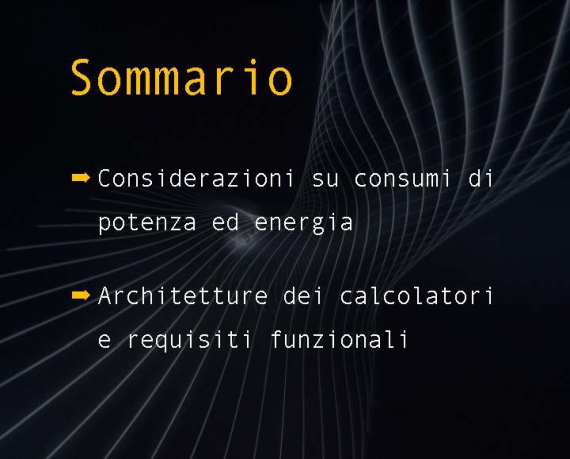
\includegraphics[width=0.40\textwidth,
                    trim=40 80 10 40, % L B R T
                    clip]
                    {images/Lez02_p01_fig_02.png}
%   \caption{Esempio wrapfig}
\end{figure}
Il sommario della presente lezione consiste nell'introdurre delle considerazioni su consumi di potenza ed energia, che sono dei fattori molto importanti per i calcolatori e affrontare il problema delle architetture dei calcolatori e dei loro requisiti funzionali.

\section{Consumi di potenza ed energia}

Negli anni questo è diventato uno dei punti più critici delle architetture dei calcolatori.
Per chi è un pochino più giovane, più anziano, ricorderà quando non era sostanzialmente importante in un calcolatore quanto esso consumasse perché il consumo complessivo era generalmente molto inferiore di una piccola lampadina.
Al contrario, negli anni i consumi sono andati via via sempre più aumentando.

\begin{figure}[H]
  \centering
  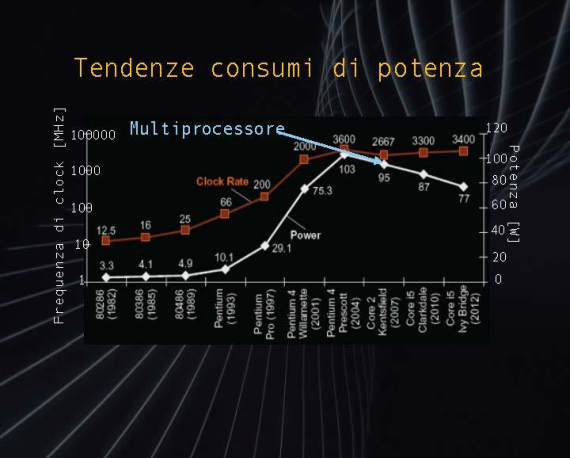
\includegraphics[width=0.8\textwidth,
                    trim=50 110 45 100, % L B R T
                    clip]
                    {images/Lez02_p01_fig_04.png}
  \caption{Consumi di potenza
  \label{fig:Lez02_p01_fig_04}}
\end{figure}


E' importante osservare il grafico \ref{fig:Lez02_p01_fig_04} che rappresenta l'andamento dei consumi dell'architettura Intel al variare del tempo.

Consideriamo sull'asse delle ascisse l'architettura Intel 286, che era ancora un'architettura a 16 bit, la prima architettura a 32 bit, il 486 che era un 386 con una unità virgola mobile, poi le prime architetture superscalari, il Pentium, il Pentium Pro e via discorrendo, fino ad arrivare a un picco dei consumi di potenza in corrispondenza delle architetture superscalari. Se ricordate la lezione precedente in corrispondenza di quella accelerazione delle performance dei processori quell'aumento delle prestazioni è venuto sia dalla regge di Moore che dall'aumento del consumo della potenza.

Come vedete negli anni 80 si consumavano poche unità di Watt e a partire dagli anni 90 c'è stata un escalation passando da poche unità di Watt fino a un centinaio di Watt agli inizi degli anni 2000, questi sono dei processori di tipo desktop, alcune architetture server hanno anche raggiunto 150 e più Watt di potenza.

La cosa che è importante osservare è che l'andamento della frequenza di clock è mostrata in scala logaritmica mentre l'evento della potenza è mostrato in una scala lineare, quindi oggettivamente la velocità del processore è aumentata molto più grazie alle leggi di Moore e al contrario la potenza è aumentata ma alla fine di circa un ordine di grandezza e mezzo.

Abbiamo già accennato che attorno a 2003-2004 si è rallentata la corsa dell'aumento delle prestazioni aumentando il paralelismo al livello di istruzioni e hanno cominciato a prendere piedi processori multicore, già qui attorno a 2004-2005 siamo in un ambiente multicore e vi accorgete che il prodotto alto di gamma di desktop Intel in questo caso tende inizialmente addirittura a scendere in velocità e poi più o meno a livellare attorno a 3,4 GHz.

Questo è però negli anni stata accompagnata a una riduzione complessiva del consumo.
Notate che il consumo è uno dei parametri più importanti sia perché se volete utilizzare un apparecchio portatile la potenza deve essere da qualche parte fornita, in questo caso di processori per architetture desktop la maggior problematica è quella della dissipazione della potenza perché questa potenza se viene dissipata deve essere anche smaltita fuori dal processore.

Notate che la legge di Moore comporta che a parità di numero dei gate l'aria scala sostanzialmente come il quadrato e quindi se non diminuisce anche la potenza contemporaneamente il processore verrebbe a scaldarsi in maniera esagerata e prima o poi arrompersi in modo catastrofico.

Quindi il fatto molto importante è osservare che con l'inversione della tendenza da aumento del paralelismo a livello di istruzioni passando alle architetture multicore si è anche cercato di ovviare al problema del continuo aumento della potenza dissipata dal singolo processore in particolare da quello che chiamiamo package.
Nella maggior parte dei casi che noi consideriamo abbiamo un multicore come singolo die, cioè singola lastrina di silicio all'interno di un package.
Esistono delle applicazioni per architetture server o di calcolo parallelo di cui spesso si è fatta avanti la IBM in cui ci sono più chip all'interno del singolo package.
Di questo non parliamo in questo istante e ce ne potremmo occupare forse un pochino più avanti.
Notate, vi ho detto, come i punti di inflessione della curva in parte corrispondono all'avvento delle architetture multicore.

\begin{figure}[H]
  \centering
  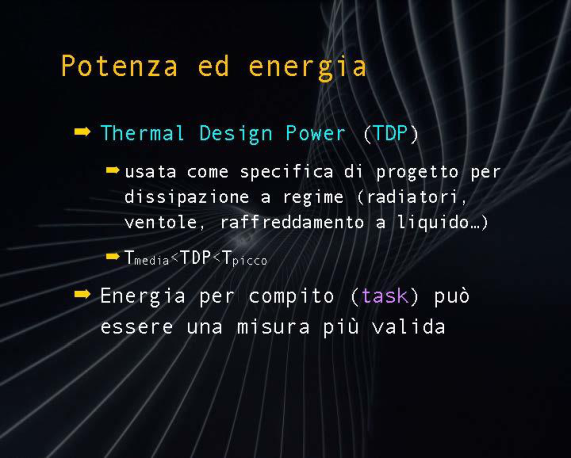
\includegraphics[width=0.6\textwidth,
                    trim=50 110 45 100, % L B R T
                    clip]{images/Lez02_p01_fig_05.png}
  \caption{Thermal design power (TDP)}
  \label{fig:Lez02_p01_fig_05}
\end{figure}

Allora, è importante però osservare quali sono i parametri che ci interessano dal punto di vista del progetto di un'architettura di elaborazione. figura \ref{fig:Lez02_p01_fig_05}.

Quello che spesso troverete scritto è il cosiddetto thermal design power o TDP.
Questa grandezza è usata come specifica di progetto per dimensionare il progetto di dissipazione a regime, in particolare l'uso di radiatori, di ventole o eventualmente di raffreddamento al liquido.
Questo è un parametro che trovate quasi sempre e oramai i processori vengono venduti specificando qual è il thermal design power, cioè la potenza che voi dovete rimuovere a regime dal package del vostro processore anche se lo zoccolo stesso contribuisce attraverso la piadinatura a dissipare parte della potenza.
In generale il TDP è compreso fra la potenza media del processore e la potenza di picco, notate che non è nell'uno, nell'altro nella generalità perché la potenza media presuppone un funzionamento generalmente non costante sono pochi casi, in genere quelli di number crunching, di calcolo numerico intenso in cui il processore lavora in continuazione, in molte situazioni, soprattutto negli utilizzi da desktop è molto raro che il processore lavori sul carico massimo per un tempo lunghissimo.

Al contrario a volte il processore può assorbire una potenza elettrica più alta della potenza dissipabile a regime e questo avviene in particolare se le temperature interne, quelle delle giunzioni, sono ancora sufficientemente basse da consentire di accumulare parte del calore in cui l'energia elettrica è stata trasformata e smaltirlo successivamente, quindi immaginate di partire con un processore a temperatura ambiente se la temperatura massima è per esempio 50° facciamo una sia molto conservativa in realtà è un po' più alta, è chiaro che finché la temperatura delle giunzioni non ha raggiunto il punto critico la potenza dissipata può essere maggiore di quella che i dissipatori consentono di dissipare, è chiaro che la maggior potenza elettrica dissipata comporta un aumento della temperatura del processore fino a che si raggiunge una temperatura critica a quel punto la dissipazione deve diminuire perché altrimenti ci potrebbero essere dei danni catastrofici nell'architettura.

Molte volte è però più importante considerare anche l'energia per singolo compito, questa può essere una misura ben più valida, immaginate  dover fare delle transazioni Facebook, Amazon, Google, per ogni transazione che voi fate il tempo di reazione non è critico, deve essere rapido perché l'utente non vuole stare ad aspettare, però se la transazione avviene in un millisecondo o due millisecondi dal punto di vista dell'utente è del tutto irrilevante, dal punto di vista dell'operatore delle architetture che compiono la transazione invece la dissipazione di potenza può essere particolarmente importante, in particolare all'azienda che fornisce quel servizio interessa sapere quant'è l'energia per singola transazione, per esempio ogni volta che voi fate un search su Google sapere quel è un'energia dissipata, sembra strano ma è un'energia abbastanza importante, chi gestisce quel tipo di macchina non si preoccupa tanto di quanto sia la potenza ma quanto sia l'energia per la singola transazione.
Consideriamo altri parametri che ci interessano per analizzare il problema figura \ref{fig:Lez02_p01_fig_06}.

\begin{figure}[H]
  \centering
  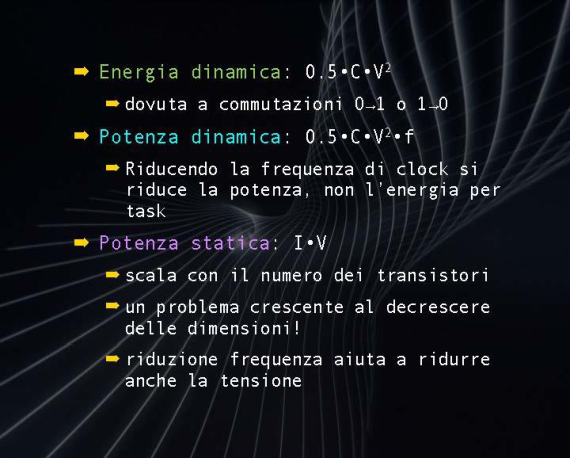
\includegraphics[width=0.6\textwidth,
                    trim=50 50 45 40, % L B R T
                    clip]{images/Lez02_p01_fig_06.png}
  \caption{Energia dinamica, Potenza dinamica, Potenza statica}
  \label{fig:Lez02_p01_fig_06}
\end{figure}


dell'energia dinamica che è calcolata come un mezzo della capacità per la tensione di carica a cui viene caricata la capacità stessa, questa è la tipica energia che serve per caricare una porta logica, una capacità C, non sarà una capacità del tutto lineare ma nella nostra approssimazione possiamo considerare una buona approssimazione e in generale la capacità massima a cui viene caricata, se per esempio V è la tensione di pilotaggio dei nostri transistori, questa energia dinamica per il singolo evento di commutazione della singola porta è calcolata come la metà della capacità per la tensione al quadrato.
Sembra un conto molto semplice ma considerate che vi saranno qualche unità di miliardo di transistori e tutto questo concorre all'evento carica delle capacità dei transistori.
In ogni commutazione questa capacità verrà caricata o scaricata e quindi vi sarà una dissipazione di energia.
Al contrario consideriamo come potenza dinamica l'energia moltiplicata per la frequenza di commutazione, se a un singolo evento corrispondono x joule di energia, se andate a 1 GHz di frequenza avrete n joule per 1 GHz e avrete quindi la potenza dinamica necessaria al caricamento delle capacità parassite delle vostre porte. Per molti anni e fino a che non si è avuto uno scaling attorno ai 130 nanometri delle dimensioni di disegno, questa era la potenza più critica nel progetto di un processore.
In generale vi accorgete che riducendo la frequenza di clock si riduce la potenza, non l'energia per task, cioè per compito svolto.
A titolo di esempio se per svolgere un search, ad esempio su Google, occorre svolgere un certo numero di istruzioni, vi accorgete che è irrilevante a che frequenza va il processore, se andasse più lento o più veloce il numero delle istruzioni rimarrebbe uguale e quindi dal punto di vista della potenza dinamica, cioè caricare e scaricare i condensatori nulla cambierebbe.
Come vi ho detto per molti anni la potenza dinamica è stata il parametro più importante di disegno.
Allo scalare delle dimensioni dei transistor sono state anche ridotti gli spessori degli ossidi, i canali sono diventati più corti e quindi ci sono state sempre più correnti di perdita, questo MOS spesso chiamato insulated gate field effect transistor, cioè transistore effetto di campo a porta isolata è diventato sempre meno a porta isolata e quindi cominciava a scorrere corrente dalla giunzione MOS stessa, cominciavano a scorrere anche delle correnti fra source e drain del transistore, al punto tale che diventa importante considerare anche la potenza statica data dal prodotto della corrente per la tensione di alimentazione dei transistor, in genere nei processori la tensione di alimentazione è oggigiorno circa 1 V.
% 12:47
La cosa importante da osservare è che la potenza statica scala con il numero dei transistori, ma non è invariante rispetto alle transazioni perché a parità di tensione di alimentazione più tempo si sta maggiore è l'energia dissipata senza fare nulla di particolare.
La cosa importante è osservare che è un problema crescente al decrescere delle dimensioni dei transistori.
In generale è vero che la potenza statica non varia con la frequenza, però la riduzione della frequenza aiuta anche a ridurre la tensione di alimentazione e quindi indirettamente anche a ridurre la potenza statica.
Vi accorgete che il progetto di un'architettura diventa quindi un fatto sempre più complicato e anche le scelte non solo di progetto del processore ma anche del suo utilizzo in condizioni applicative fa sì che a volte bisogna fare delle scelte, delle scelte di progetto, delle scelte a volte di compromesso, spesso si cerca di fare delle scelte che possano essere flessibili rispetto alle variazioni delle necessità stesse ed questo di cui ci occupiamo in questa lezione e nella successiva.

\begin{figure}[H]
  \centering
  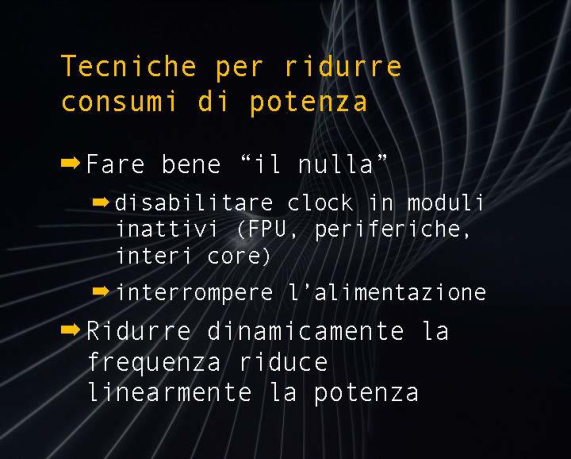
\includegraphics[width=0.6\textwidth,
                    trim=40 40 45 40, % L B R T
                    clip]{images/Lez02_p02_fig_01.png}
  \caption{Tecniche per ridurre i consumi di potenza}
  \label{fig:Lez02_p02_fig_01}
\end{figure}

Consigliamo delle tecniche per ridurre i consumi di potenza fig. \ref{fig:Lez02_p02_fig_01}
%15:48
Il primo caso è sempre quello di fare bene il nulla.
Cosa intendo per fare bene il nulla?
In molti casi un processore deve fare delle funzioni e a un certo punto smette di farle perché ha finito di fare il compito.
Immaginate ad esempio il vostro telefonino che è un'architettura di elaborazione.
Il vostro telefonino può passare da picchi di carico molto importanti come una compressione video a situazioni dove non fa praticamente niente, l'avete lasciato lì bello sul tavolo e ad esempio avete disabilitato la parte radio quindi il telefono non deve neanche andare a inseguire il canale, il segnale, più o meno legge un orologio e aggiorna l'orologio e quindi consumerebbe veramente poco.
Quindi quello che è importante è che il vostro telefono nelle funzioni, nei momenti in cui non è chiamato a fare compressione video, compressione audio, decodifica video, decodifica audio o altre funzionalità per esempio navigare su internet o comunque tutti gli algoritmi di criptografia che ci sono dietro la trasmissione cellulare, è importante che sappia bene fare bene il nulla, cioè consumare poco a riposo.
Per fare questo spesso fra le varie funzionalità si disabilita il clock in moduli inattivi, per esempio nella floating point unit, nell'unità a virgola mobile, in alcune periferiche o addirittura in interi core.
L'esempio è caratteristico, se voi dovete semplicemente aspettare con il vostro sistema, il vostro telefonino, il vostro calcolatore embedded o il vostro desktop di tanto in tanto una comunicazione attraverso una porta esterna, in quel caso l'unità a virgola mobile verosimilmente non dovrà essere utilizzata, bisognerà semplicemente gestire un po' di interrupt dalle esterni per cui l'unità etnetica e logica e l'unità di controllo bastano e avanzano, quindi l'unità a virgola mobile potrà essere disattivata.
Il primo livello di disattivazione è quello di non far passare il clock, il quale per sua natura determina una potenza dinamica, come vi ho detto nelle slide precedenti, importante perché quelle capacità dovranno essere caricate e scaricate a ogni transizione del clock.
Inoltre è possibile anche interrompere completamente l'alimentazione dai moduli che non occorre.
Infine si può giocare riducendo dinamicamente la frequenza e ridurre dinamicamente la frequenza consente di ridurre linearmente la potenza dissipata in base alle formule che vi ho dato prima.
Questo gioco dell'interruzione dell'alimentazione in linea di principio non viene a costo zero, nel senso che bisogna dimensionare opportunamente dei transizioni come degli interruttori complessivi dell'alimentazione, quindi l'implementazione fisica diventa un po' più complessa, molte volte è vantaggiosa, altre volte non viene utilizzata, oppure viene utilizzata in certe particolari condizioni.
Perché?
Perché notate che dover ridistribuire la potenza comporta quindi comunque dei tempi, ad esempio una maggiore o minore carica di alcuni condensatori, ad esempio quelli di blocco, quindi questo in generale richiede un po' più di impegno sia in termini di tipo progettuale che di gestione del software, perché un'unità a cui è stata interrotta la potenza ci rimette un po' di più a riattivarsi, un'unità a cui è stata o semplicemente disabilitato il clock, che ci mette ovviamente molto di più di un'unità a cui non è stato per niente disabilitato il clock, la quale risponde al prossimo ciclo di clock come qualunque macchina sequenziale.
In ultima riga vi ho detto anche che si provvede a ridurre dinamicamente la frequenza e in realtà il risparmio di potenza è più che lineare, nel caso si riduca la frequenza, perché come vi ho già accennato, ridurre la frequenza può consentire anche di ridurre la tensione di alimentazione che in sua volta riduce sia la potenza statica che la potenza dinamica ed è quello che spesso avviene nella maggioranza dei processori, sia desktop che per applicazioni portati dove la potenza è importante sia in termini di disponibilità di energia nelle batterie, sia in termini di dissipazione della potenza stessa, perché ad esempio nessuno di noi vorrebbe una voluminosa ventola montata sul nostro bellissimo telefonino o nel nostro bellissimo smartphone.
Abbiamo alcune delle tecniche per ridurre ancora i consumi di potenza per processi ad esempio non ben parallelizzati, si procede all'incremento di frequenza di clock di 1 o più core e contemporaneamente si disabilitano i core inattivi.
Questo ragionamento sembra essere in contrasto con quello che vi ho detto, cioè con la tendenza di avere sempre più core e una frequenza decrescente, ma considerate che non tutti i processi sono facilmente parallelizzabili o semplicemente sono dei processi che sono stati scompilati anni prima senza tener conto dell'esistenza di più core e quindi non sono più parallelizzabili e che avete soltanto il codice macchina.
Quindi in quei casi se volete effettivamente avere una migliore efficienza, cioè maggiori prestazioni e minori consumi, non vi resta altro che spegnere i core non utilizzati perché non utilizzabili da quel codice e aumentare nei limiti del possibile la frequenza dei clock in uso, la frequenza dei core in uso.
Infine è utile gestire stati a bassa potenza sia per le drum che per i dischi, quindi i dischi magnetici vengono messi ad esempio con le testine in parcheggio, cioè il disco viene fermato e così rispiemete qualche Watt di potenza.
Vi do adesso uno spunto per la riflessione e vi invito a riflettere per le diverse classi di calcolatori elencando cause e criticità della dissipazione di potenza.
Ovviamente questo torneremo avanti nel corso ma è importante che voi vi fermiate un attimo, cerchiate di riflettere su quali possono essere le cause soprattutto quali siano le criticità nelle diverse classi di calcolatori che conoscete o che venite progressivamente a conoscere.
Ponetevi sempre queste domande perché non è un dettaglio irrilevante.
Continuiamo quindi con il prossimo argomento, cioè le architetture dei calcolatori e i requisiti funzionari.
L'approccio classico alle architetture dei calcolatori è la cosiddetta instruction set architecture, cioè il repertorio istruzioni dell'architettura o ISA o AIS se volessimo pronunciarla più correttamente in inglese.
Questo è un acronimo che utilizzeremo nel proseguio.
Vi invito a seguire il corso della laurea di primo livello in cui l'argomento è stato trattato con un certo livello di approfondimento.
Tipicamente in una ISA si considerano gli registri, i modi di indirizzamento della memoria, le operazioni disponibili nel repertorio e gli operandi, il controllo del flusso di istruzioni e il modo in cui le istruzioni sono codificate, cioè la codifica dell'istruzione all'interno della parola istruzione.
Sempre nell'approccio classico altri aspetti vengono posti in secondo piano e vengono chiamati in modo implicitamente riduttivo implementazione.
Questo invece è particolarmente importante.
Continuiamo sull'argomento e consideriamo un esempio che nelle architetture l'indirizzamento è per byte e perché risulta conveniente indirizzare individualmente ciascun byte, ma l'indirizzamento del singolo bit non viene fatto perché richiederebbe più linee.
Nell'evoluzione storica dove anche le piste erano importanti ha fatto sì che ci si è stabilizzati come elemento minimo indirizzabile indipendentemente al byte e non al bit e non al nibble.
Questa è una scelta e in alcuni casi uno potrebbe addirittura lavorare direttamente solo sulla parola, in alcune architetture, ad esempio i digital signal processors, questo a volte viene fatto ma non è molto comune.
In generale è importante osservare che si indirizza per byte.
Le locazioni dei byte hanno quindi indirizzi progressivi, zittati indirizzi progressivi 0, 1, 2 fino a 2 alla k, 2k meno 1, se k sono il numero degli locazioni.
Per parole di 32 bit le locazioni di memoria hanno sempre indirizzi 0, 4, 8 e così via, cioè multipli di 4.
Consideriamo quello che viene chiamato indirizzamento crescente o indirizzamento decrescente.
Si dice indirizzamento crescente o big-endian in inglese quello che assegna gli indirizzi inferiori ai byte meno significativi della parola.
L'indirizzo decrescente o little-endian usa l'ordine opposto.
Alcuni processori usano o l'uno o l'altro ma in alcuni particolari i processori sono anche supportati entrambi i modi, in quel caso i processori vengono detti by-endian.
La scelta della modalità dell'indirizzamento crescente o decrescente, quindi cioè little-endian o big-endian in questi processori viene fatto spesso esclusivamente in fase di avvio mediante il controllo per esempio di un apposito piedino che consente quindi al processore di poter correttamente interpretare gli indirizzi.
Forse la definizione non vi è così intuitiva, penso che un esempio sia la cosa più semplice.
Considerate quindi qui una parola di 32 bit, 4 byte, questi sono indirizzi dei byte, nel caso del big-endian e il byte più a sinistra quello che definisce l'indirizzo della parola, cioè il byte di peso più significativo, questo è il byte di peso meno significativo, al contrario nel caso del little-endian e l'indirizzo del byte meno significativo, cioè del little, del piccolo, che definisce l'indirizzo della parola.
La parola successiva sarà, ad esempio se la prima è a 0, la seconda sarà 4, che corrisponde ancora all'indirizzo del byte meno significativo.
Questo è utile da sapere perché spesso anche molti software, molti codici, i dati vengono memorizzati per semplificare il processamento dei byte.
Se andate a vedere la codifica di alcuni algoritmi di compressione video o di immagine, questo viene messo, ad esempio il TIFF è uno tipico di questo in cui voi potete scegliere l'ordinamento dei byte che rappresentano le parole, l'indirizzo dei file.
Questo perché alcuni architettori leggono più facilmente una modalità invece che l'altra.
Gli indirizzi per parole di 32 bit però sono sempre a 0, 4 o 8, quindi indipendentemente da fatto se siano big-endian o little-endian, l'indirizzo è sempre a multipli di 4.
Quello che cambia è l'indirizzamento dei byte della parola rispetto ai byte e il modo in cui questi possano essere più rapidamente gestiti del processore o dove si debba agire sul singolo byte.
I bit nei byte sono sempre etichettati b7, b0 da sinistra a destra, quindi indipendentemente da tutto all'interno di un byte l'ordine è sempre lo stesso.
Consigliamo quello che viene chiamato allineamento di parola.
Gli indirizzi delle parole si dicono allineati se corrispondono a multipli del numero di byte in una parola.
Ad esempio se una parola è fatta di 2 byte gli indirizzi sono 0, 2 o 4, 6 di 4 byte 0, 4 o 8, 6 di 8 byte come ad esempio in un double precision floating point, 0, 8, 16 e così via.
Qualche processore gestisce anche indirizzi disallineati, ma spesso questo comporta incremento del numero dei cicli di accesso alla memoria.
Tipicamente alcune architetture ad esempio l'ARM consente l'accesso disallineato di 2 byte, cioè alla mezza parola, questo però non è che viene a costo 0, viene al costo di un ciclo di clock in più, cioè c'è un buffer di riordino interno che consente di accedere anche alle mezze parole.
Il motivo per cui l'ARM consente anche l'utilizzo di 16 bit verrà chiarito più avanti nel corso delle lezioni.
Vediamo ad esempio il confronto tra i cosiddetti SISC e RISC, RISC sta per Reduced Instruction Set Computer ed è un'architettura caratterizzata dall'essere load store.
Non importa quante sono le istruzioni, se le istruzioni sono semplici o complesse, semplici e complesse sono delle definizioni più diciamo filosofice che sostanziali, quello che conta è l'architettura load store, cioè l'unica operazione che si fanno, scusate, sulla memoria sono operazioni di caricamento di immagazzinamento.
Al confronto le cosiddette architetture SISC sono delle architetture di tipo load operator, cioè sono possibili operazioni direttamente sugli operandi in memoria, quindi queste agiscono solo su registri e queste agiscono sia su registri che su memoria.
I modi di indirizzamento dei RISC vi do quelli più comuni e quelli sempre esistenti, il modo immediato in cui la sintassi assemblativa si dà direttamente il valore, l'operando e il valore segnato nel campo.
Il modo registro in cui la sintassi assemblativa vi dà il valore di un registro e l'indirizzo effettivo, l'effective address in inglese, è dato dal registro stesso.
Il modo assoluto è dato da una locazione in memoria, cioè l'indirizzo effettivo è dato dal contenuto della locazione in memoria.
Indirizzamento in diretto da registro, quindi nella sintassi assemblativa in alcuni casi si usano le parentesi tonde per rappresentare R.I.
E l'indirizzo viene pescato in un registro e quindi il contenuto di quel registro diventa l'indirizzo effettivo.
E' possibile anche un modo indice e spiazzamento in cui X è lo spiazzamento, R.I.
È l'indirizzo e l'indirizzo è efficace e dato dal contenuto di R.I.
Più il valore dello spiazzamento che è una costante X.
Infine con registro base e registro indice, di fatto l'indirizzo effettivo è dato dalla somma dei contenuti dei due registri.
Esistono anche delle variazioni che qui non vi mostro in cui si può mettere uno spiazzamento in aggiunta ai due registri e quindi l'indirizzo è efficace, effettivo scusate, non è altro che la somma dei contenuti dei due registri più lo spiazzamento.
In generale questo modo X.R.I.R.J.
È quello più generale perché se si mette come X zero si ha il base con indice, se si mette uno dei due registri a zero si ha indice spiazzamento, se si mette uno dei due registri e lo spiazzamento a zero si ha l'indirizzo, l'indiretto da registro.
Nel caso dei SISC vi sono anche altri modi di indirizzamento, il modo relativo, relativo in questo caso è il program counter quindi è un modo con indice dove il registro indice non è altro che il program counter.
L'autodecremento e l'autodincremento sono particolarmente interessanti perché in una singola operazione apparentemente il processore è in grado sia di calcolare l'indirizzo effettivo leggendo il contenuto del registro e immediatamente aggiornare il contenuto del registro e aumentandolo di uno.
L'autodecremento è analovo in cui prima si decrementa il contenuto del registro e poi si ottiene il registro.
Notate che queste operazioni non sempre riescono ad avvenire un singolo colpo di clock, per una più attenta analisi dei flussi di calcolo vi rimando al corso del primo livello in cui questo argomento è stato trattato con un certo dettaglio.
Passiamo a considerare lunghezza fissa e variabile delle istruzioni.
Come vi ho detto i RISC hanno tipicamente istruzioni lunghe di 32 bit ma esistono delle situazioni in cui è utile impacchettare istruzioni più piccole.
Perché non facciamo sempre istruzioni più piccole?
Perché le istruzioni più piccole spesso vengono con una penalità.
Per esempio lo vedremo quando tratteremo l'architettura ARM ma come ho detto alcuni RISC come l'ARM e anche lo stesso MIPS hanno la possibilità di utilizzare istruzioni a 16 bit.
Queste istruzioni non sono mischiate contemporaneamente, cioè nello stesso codice con le istruzioni a 32 bit.
Vi sono due stati diversi del processore.
Uno che è in grado di interpretare istruzioni a 32 bit e un altro stato che è in grado di interpretare istruzioni a 16 bit.
Ma per compiti poco onerosi dal punto di vista computazionale ma dove la quantità di memoria è vincolante si può ricorrere a queste istruzioni a 16 bit.
Nel caso dell'ARM vengono chiamate TAMB come nome per definirle.
Il caso opposto è quello delle istruzioni di architettura intera a 32 e 64 bit.
Nella 64 bit ci sono due diverse implementazioni.
Queste hanno istruzioni di lunghezza variabile.
I suzioni variabile quanto?
Tipicamente da 1 a 12 byte.
Quindi alcune istruzioni possono essere molto brevi, altre istruzioni possono essere veramente lunghe.
Si usano quelle che vengono chiamate i prefix nelle istruzioni e fanno sì che la decodifica di queste istruzioni sia tutto tranne che semplice elementare come abbiamo visto nel corso del primo livello sull'istruzione di decodifica di una istruzione RISC.
Vi ho accennato già nella prima lezione che però l'overhead della decodifica delle istruzioni di un repertorio SISCHE è venuto a perdersi col passare del tempo.
Consideriamo invece al contrario ora quello che viene chiamato un approccio holistico.
Questo approccio non tiene più conto solo dell'architettura delle repertorie istruzioni ma considera i requisiti specifici di una macchina obiettiva.
Noi dobbiamo disegnare una macchina, cioè un'architettura di elaborazione che abbia un preciso obiettivo.
Deve essere un telefonino cellulare, deve essere un netbook, deve essere un desktop, deve essere una software house, deve essere un supercalcolatore.
Quindi il requisito va preso complessivamente, non è che ci si può limitare alla solo repertorio istruzione e occorre ad esempio cercare di fare un progetto per massimizzare le prestazioni e i limiti dei vincoli.
I vincoli possono essere il costo dei componenti, la potenza dissipata, la disponibilità del sistema, cioè quanto questo sistema sia robusto rispetto a problemi.
Per esempio se dovete fare un server di dati, per esempio vi interesserà che anche se si rompe uno dei dischi il sistema continui ancora a fornire il servizio.
Se avete per esempio il gestore dei bankomat di una banca, capite quanto è importante che la disponibilità sia continua.
Se gestite un portale di vendita e quello che certamente non volete è che vi si rompa il portale di vendita soggetto a sovraccarico nei giorni immediatamente precedenti natale, quando la maggior parte degli acquisti, i regali e quant'altro viene fatto.
All'interno di questo approccio listico noi consideriamo tutto, consideriamo chiaramente anche l'instruction set architecture, consideriamo la microarchitettura con cui questa isa è implementata e alcuni dettagli dell'hardware che andiamo a definire più avanti.
Cos'è l'organizzazione di un calcolatore?
A volte trovate il termine organizzazione, altre volte trovate il termine microarchitettura.
Alcune isa possono essere implementati con diverse microarchitetture, ad esempio possono essere implementate da diversi produttori AMD e Intel, vi ho raccontato come durante la guerra RISC-SISC degli anni 90, a un certo punto AMD ha cominciato a implementare delle architetture, il repertorio di istruzioni Intel all'interno con un'architettura RISC trascodificando di fatto le istruzioni Intel nelle istruzioni native dei suoi processori.
Similmente ha fatto Intel, ma il modo in cui queste microarchitetture sono state realizzate sono del tutto diverse fra AMD e Intel.
Ma anche lo stesso produttore, tanto per fare un esempio, Intel ha evoluto le sue microarchitetture, per esempio negli anni in cui vi sto parlando, l'Ivy Bridge e l'Aswell sono due variazioni evolutive della stessa microarchitettura, ma non sono più identiche.
A volte le microarchitetture possono essere radicalmente diverse, ma non sono più identiche.
A volte le microarchitetture sono radicalmente diverse pur supportando lo stesso ISA, questo per esempio per differenziare i desktop o i server, nel caso dell'Ivy Bridge e dell'Aswell, dall'ATOM per le applicazioni mobili o dall'Intel PHY per le applicazioni di calcolo ad alte prestazioni, high performance computation.
In generale poi la microarchitettura può essere customizzata da chiunque prende in licenza l'ISA dal proprietario dell'ISA e eventualmente una descrizione register transfer logic.
Questo è quello che avviene tipicamente con ARM, cioè voi pagate una licenza all'azienda ad ARM e acquisite il diritto o ad utilizzare solo l'instruction set architecture o addirittura prendete il register transfer logic description del microprocessore.
Vediamo cosa si intende per hardware.
Si riferisce al dettaglio dell'implementazione della logica, quindi stesso ISA, stesso microarchitettura, ad esempio lo stesso Intel Aswell, ma differente di un altro.
Ci sono due porti, numero di cores, 2, 4, 8, 16, numero dei livelli di cache, le 1 e le 2, a volte anche 1 e le 3, dimensioni della cache, tipo il numero di periferiche, se via il quick pack interconnect, quante porte PCI express, quante porte USB, quante SATA, la gestione della memoria se con o senza codici di correzione d'errore.
E questi vengono dei desktop servers e high performance computing.
Vi do ora il solito spunto per la riflessione e vi chiedo perché non è sufficiente limitarsi a considerare l'ISA e la frequenza di clock nella valutazione della scelta di un processore.
Quello che molti ragazzi fanno, compro il processore calcolatore più veloce, prendo il clock più veloce e non me ne preoccupo.
Se volete riflettere su quello che già vi ho detto, apritevi e createvi dei dubbi, li risolveremo in parte nelle lezioni successive, ma è importante voi che vi poniate il dubbio di non ragionare sempre, certamente solo su un solo parametro, il clock più veloce o più core e basta.
Con questo vi saluto e vi rimando alla continuazione dell'argomento nella prossima lezione.
\chapter{Lezione 3 - Approccio quantitativo al progetto e all'analisi. Parte 3}

Continuiamo l'argomento dell'approccio quantitativo al progetto e all'analisi, al progetto e all'analisi di architetture di elaborazione.

\FloatBarrier
\begin{figure}[H]
  \centering
  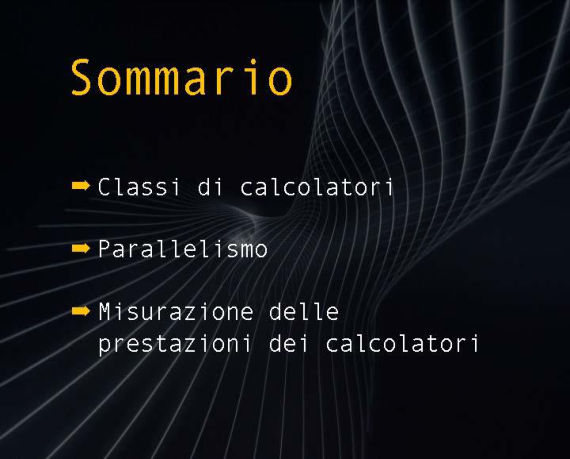
\includegraphics[width=0.40\textwidth,
                    trim=40 80 10 40, % L B R T
                    clip]
                    {images/Lez03_p01_fig_02.png}
  \caption{Sommario}
  \label{fig:Lez03_p01_fig_02}
\end{figure}
\FloatBarrier
\noindent

Fra le classi di calcolatori vi faccio un rapido richiamo al fine di avere un linguaggio comune.

\FloatBarrier
\begin{figure}[H]
  \centering
  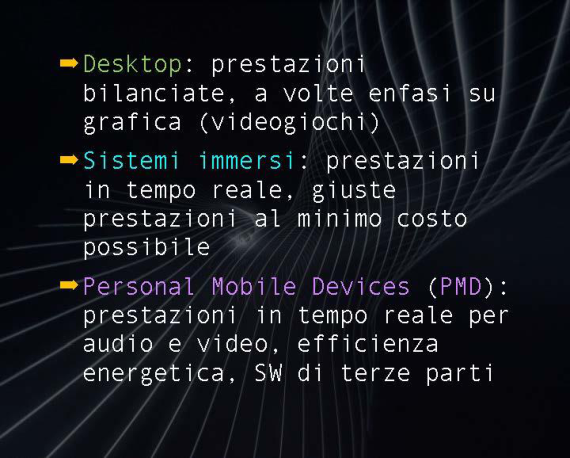
\includegraphics[width=0.40\textwidth,
                    trim=40 50 10 40, % L B R T
                    clip]
                    {images/Lez03_p01_fig_04.png}
  \caption{Sommario}
  \label{fig:Lez03_p01_fig_04}
\end{figure}
\FloatBarrier
\noindent

Definiamo desktop, quei calcolatori da tavolo, quelli che storicamente sono stati personal computers, sono caratterizzati da prestazioni bilanciate a volte c'è enfasi sulla grafica, cioè sui videogiochi.
Questo è il classico computer da casa, da ufficio, oramai un'architettura multicore, per i motivi che vi ho raccontato nelle lezioni precedenti.
Spesso è un'architettura multicore, ma più che i core del microprocessore, quelli che più interessano sono gli elementi grafici, perché spesso vengono utilizzati come delle piattaforme di gioco o per altre attività multimediali nelle mura domestiche.
Spesso è uno spreco di risorse di calcoli e comunque la definizione di prestazioni bilanciate significa che né si esaltano le prestazioni, né si esalta il risparmio di potenza, perché nel primo caso non è necessario avere prestazioni di calcolo necessariamente al massimo, nel secondo caso essendo dei dispositivi attaccati all'alimentazione di rete e generalmente anche abbastanza spaziose all'interno è possibile utilizzare come metodo di raffeddamento con radiatori e ventole che possono tranquillamente rimuovere potenza nell'ordine del centinaio di watt.
Se ricordate il grafico della lezione precedente, più o meno quelle sono le potenze.
Siamo che al momento i desktop di ultima generazione hanno un TDP attorno ai 77 watt.
Come vi ho detto questa è stata una potenza che è scesa rispetto ai picchi di pochi anni fa, ma comunque si tratta di potenze non completamente trascurabili e come se andate a aprire una scatola vi accorgete immediatamente che internamente vi sono anche dei corposi radiatori e delle ventole montate.
Se vi volete sbizzarrire nel vedere l'andamento delle potenze e delle temperature ci sono delle utility di sistema o di terze parti spesso che vi consentono di farlo.
È molto illuminante vedere questo.
Un esempio sotto Windows potrebbe essere CPU Z che vi permette di vedere molte di queste caratteristiche.
Capire cosa si intende per prestazioni bilanciate, a quanto va la frequenza del clock, a che tensione lavora il processore e generalmente la potenza che esso dissipa.

Altri sistemi sono i cosiddetti sistemi immersi che è una brutta traduzione dell'inglese embedded systems e sono tutti quei sistemi caratterizzati generalmente da prestazioni in tempo reale, giuste prestazioni al minimo costo possibile.
Ovviamente giusto è un termine soggettivo, quello che intendiamo con questo aggettivo è quello di dire che i sistemi embedded, li chiameremo sempre embedded systems o sistemi embedded perché il sistema è immerso in un termine molto poco utilizzato nella comunità, intendiamo quei sistemi che sono dedicati a una particolare funzione.
Embedded system può essere qualunque cosa, dal controllore della vostra lavatrice a un sistema come un router di rete, in qualche modo anche a una console per videogiochi, anche se una console per videogiochi sia un desktop o un sistema immerso è un po' grigio come intervallo perché molte funzionalità di queste console sono di fatto quasi equivalenti a quelle di un desktop anche se è un po' meno general purpose, cioè ha uso meno generale. Però ad esempio con una molte console potete navigare, vedere filmati, vedere DVD e così via.
La cosa caratteristica che descrive i sistemi immersi è che tecnicamente sono dei sistemi chiusi, cioè non sono modificabili o non è possibile caricare su essi dei programmi prodotti da soggetti diversi dal prodotto del sistema immerso tal quale, per questo vi ho detto che anche ad esempio una console è un po' grigio perché alcune cose possono girare e non necessariamente tutto.

Una particolare categoria di sistemi embedded possono essere i cosiddetti personal mobile devices, le caratteristiche più importati sono le prestazioni in tempo reale per audio e video, l'efficienza energetica e la possibilità di far girare software di terze parti.
L'ultima di queste caratteristiche, la possibilità di far girare software di terze parti, li rende sostanzialmente diversi dai sistemi embedded di tipo convenzionale.
In qualche modo sono al confine fra un personal computer di tipo portatile e un sistema immerso. La caratteristica fondamentale che possono far girare i software di terze parti è che hanno delle innovative modalità di input e di output che abbiamo discusso nelle due lezioni fa, ma in tutta sostanza sono dei calcolatori embedded che hanno un insieme di funzionalità abbastanza ottimizzate per uno specifico impiego.
Sono un po' meno general purpose anche se in alcuni di essi è possibile utilizzare delle porte esterne, per esempio una porta USB per ad esempio pilotare appositi ulteriori dispositivi o lo si può fare anche in modalità wireless.
Fra i personal mobile device vi ricordo quelli che utilizzate comunemente, gli smartphones, i tablets e i loro ibridi, cioè i phablets, quella categoria di piccoli tablet o grandi smartphone, indicativamente attorno ai 5-6 pollici di diagonale che ultimamente stanno prendendo abbastanza piede e che al crescere delle dimensioni vedono sempre meno critiche le esigenze, i vincoli di natura di efficienza energetica, ma comunque qualunque utente vorrebbe poter utilizzare liberamente questo tipo di PMD nell'arco di almeno un'intera giornata e vi accorgete spesso che quando sono più compatti questo risulta particolarmente difficoltoso.

%07:12

\FloatBarrier
\begin{figure}[H]
  \centering
  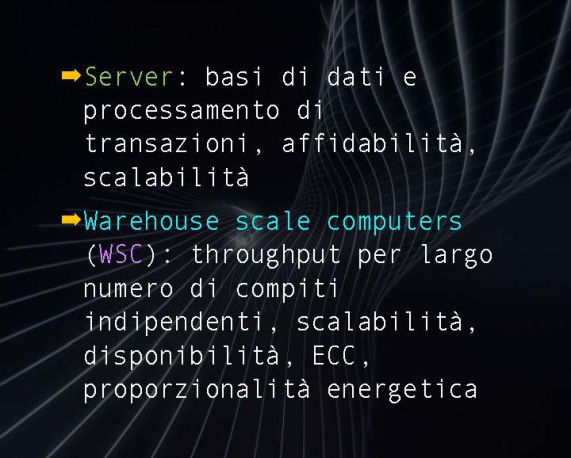
\includegraphics[width=0.40\textwidth,
                    trim=40 80 10 40, % L B R T
                    clip]
                    {images/Lez03_p01_fig_05.png}
  \caption{Sommario}
  \label{fig:Lez03_p01_fig_05}
\end{figure}
\FloatBarrier
\noindent

A un altro estremo troviamo i server, sono utilizzati per basi di dati e per processamento di transazioni caratterizzati da affidabilità e scalabilità.
Nel caso dei server immaginate una transazione di una banca, la fidabilità è fondamentale, ma anche la scalabilità perché se aumentano il numero di sportelli di Bancomat il sistema deve poter essere per esempio scalabile.
Una specie di estremo dei server è il cosiddetto warehouse scale computers, cioè quei computer di grande dimensione interconnessi per cui il throughput per un largo numero di compiti indipendenti è una caratteristica fondamentale, rimane ancora la scalabilità, la disponibilità del sistema, vi ho fatto l'esempio del transazione di natalizia e di acquisto, la correzione d'errore perché non si vuole per esempio che in una transazione vi sia un errore nella registrazione per esempio del conto su cui accreditare l'attività e la cosiddetta proporzionalità energetica che è una caratteristica annessa alla scalabilità.
Cosa si intende per proporzionalità energetica?
Si intende che se si aumenta per esempio del 10% la capacità di calcolare e di gestire transazioni, il consumo di energia non deve aumentare di più del 10%.
Questo è molto importante perché chiaramente il costo energetico sia in termini di bolletta energetica per far funzionare le architetture di costo energetico e di elaborazione, sia per smaltire il calore, sono spesso una voce molto importante del costo complessivo della gestione di queste warehouse scale computers, cioè questi sono computer alla fine interconnessi fra loro ma in un modo scalabile, in modo proporzionalmente energetico, in maniera tale che manifesti un elevato tasso di disponibilità perché la perdita ad esempio di un singolo nodo non deve pregiudicare in nessun modo il funzionamento complessivo della piattaforma.
Vi faccio i classici esempi, Amazon, Google, Facebook, non volete che sia a un certo punto una delle macchine che fare transazioni abbia un danno, una ruptura di un disco, la bruciatura di un processore, di una zocca di memoria e così via, non vi potete aspettare che tutta Facebook smetta di funzionare, quindi in quei casi è necessario disegnare queste warehouse scale computers opportunamente.
È anche interessante al titolo di Cronaca che considera il fatto che ormai molte di queste warehouse scale computers non vengono più poste presso la sede dell'azienda stessa ma in locazioni ambientalmente favorevoli.
Quali sono le locazioni ambientalmente favorevoli?
Quelle ove l'energia elettrica costa poco e quelle ove è possibile facilmente smaltire il calore resito e quindi tipicamente l'Islanda o il nord degli Stati Uniti o del Canada nel caso in cui le aziende preferiscono mantenere nello stesso Paese dati sensibili.
Considerate che la gestione di questi dati è molto importante, vi sono anche delle importanti agenzie di intelligence che spesso accedono senza che voi sappiate, quindi state molto cauti su quello che andate a mettere sui siti social, su quello che andate a scrivere perché c'è sempre qualcuno, qualche intruso che ascolta.
Comunque quello su cui noi ci fermiamo in questo corso non ci interessiamo di sicurezza dei dati ma invece ci interessiamo maggiormente della dimensionamento del nostro sistema.
Quindi vi ho detto, siccome un sistema consuma potenza è importante pagare una bolletta energetica più economica ed è importante per esempio semplicemente ventilare senza dover utilizzare dei condizionatori.
Immaginate la differenza fra dove smaltire il calore, per esempio nel sud degli Stati Uniti, in Sicilia visto che siamo in Italia, oppure smaltirlo nel nord della Scandinavia, in Islanda in Greenlandia, cioè in quei posti dove l'aria è sempre abbastanza fresca anche nel caso di massima temperatura.
I casi esempio dell'Islanda sono anche legati al fatto che l'energia elettrica è a buon mercato grazie al geotermico.
Altri paesi, esempio il Canada, hanno una ampia disponibilità di idroelettrio, quindi in certi paesi l'energia elettrica costa meno, quindi in quei paesi è conveniente mettere dei servizi fortemente energivori come possono essere per esempio le warehouse scale computers dove ci sono spesso anche molte potenze di molte decine di megawatt impiegate per la gestione della struttura.
Provate a fare un conto sulla bolletta.
Un caso particolare di macchine di calcolo sono i supercomputer e i cluster per calcolo ad alte prestazioni, quello che in inglese si chiama high performance computing o HPC che abbiamo già utilizzato precedentemente come acronimo.
La caratteristica di questi consiste nel cercare di eseguire molte operazioni, esempio quindi servono delle F più veloci, cioè delle floating point unit veloci, quindi parallelismo a livello dati, memoria di grande dimensione e con banda elevata e inoltre intercomputing connessioni a bassa latenza ed elevata a banda.
Con questo vi do un piccolo spunto per la riflessione e vi invito a pensare in quale classe di calcolatori la latenza delle comunicazioni fra core e nell'accesso alla memoria è più critica e perché.
Questo passiamo al prossimo argomento e introduciamo il concetto di parallelismo.
Le classi di parallelismo dal punto di vista delle applicazioni possono essere divise in quelle che viene chiamate in inglese il data level parallelism, cioè il parallelismo a livello di dati o il task level parallelism, cioè il parallelismo a livello di compito.
Questo dal punto di vista delle applicazioni.
Le classi di parallelism invece dal punto di vista dell'architettura vengono classificate in instruction level parallelism, quindi a livello di istruzione.
Fra queste consideriamo le unità vettoriali o unità di processamento grafico, graphic processor units, quelle che voi conoscete il GPU, per fare calcoli grafici ma anche per fare calcoli numerici importanti dove il levato livello di parallelismo può consentire accelerazioni notevoli rispetto ai processori di tipo general purpose.
Il cosiddetto thread level parallelism, cioè quello a livello di trama.
Parleremo di questo livello di parallelismo molto nel dettaglio nelle lezioni più successive.
Infine il cosiddetto request level parallelism, cioè il parallelismo a livello di richiesta della transazione.
Vi introduco una definizione, quella che viene chiamata tassonomia di Flynn.
Questo approccio fu introdotto ormai parecchi decenni fa ma la comunità scientifica e tecnica la usa con grande frequenza.
Chiamiamo, consideriamo le cosiddette single instruction stream, single data stream o SIST, cioè un'architettura che svolge operazioni su un singolo flusso di istruzioni, su un singolo flusso di dati.
Cioè questo è il classico calcolatore che abbiamo visto nei corsi del primo livello, vi è fatta una sola istruzione alla volta senza pipeline, senza parallelismi, senza nulla di particolare, cioè c'è un dato, c'è un flusso di istruzioni.
La fase successiva è il cosiddetto single instruction stream, multiple data stream, cioè via un singolo flusso di istruzioni ma quelle istruzioni agisce su un insieme di dati.
Per esempio una delle cose più semplici è un'architettura vettoriale dove ad esempio facciamo una add fra gli elementi di un vettore e gli elementi di un altro vettore, in questo caso immaginiamo ad esempio di avere una cosa molto semplice, un vettore fatto di 4 parole di interi che viene sommato su un altro vettore di 4 parole di interi.
L'istruzione è un add vettoriale in cui parola per parola vengono sommate e vengono messe in un terzo registro, anch'esso in questo caso della dimensione di 4 parole 128 bit, il che consente con una singola istruzione, un singolo flusso di istruzioni di eseguire istruzioni su più flussi di dati in parallelo.
Esistono molte implementazioni di questa architettura SIMD nelle estensioni multimediali, ad esempio nell'intel le prime MMX, le varie versioni di SE, le più moderne AVX, nell'ARMA il neon, nell'architettura Power l'Altivec, tutte unità con varie versioni, con vari livelli di parallelismo che agiscono su flussi paralleli, da un minimo di 64 bit dell'MMX fino alle versioni più avanzate dell'AVX2 che agiscono su 512 bit.
Questo consente di aumentare notevolmente il throughput di esecuzione senza aumentare né la quantità di istruzioni, quindi la dimensione del codice, né in linea di principio aumentare i tempi, però ovviamente nulla viene esattamente a costo zero.
Un altro tipo di esempio di SIMD sono le unità di processamento grafico dove le operazioni vengono fatte su unità di memoria che rappresentano i colori dei modelli, passeremo anche su questo più avanti.
Procedendo nella tassone nuovamente FLEAM esistono i cosiddetti multiple instruction stream, single data stream o MIMD anche se di questo non vi è nessuna implementazione commerciale, è troppo pesante da realizzare, i vantaggi sono modesti.
Rispetto ad esempio allora andare nella massima generazione cioè il multiple instruction stream, multiple data stream o MIMD che può essere classificato in MIMD fortemente accoppiati o MIMD debolmente accoppiati.
Su queste classificazioni torneremo più avanti, notate che in questo caso è un'architettura parallela che fa cose diverse su flussi di dati diversi e li fa in simultanea.
Non è semplice ovviamente da gestire, l'esempio che vi ho fatto di una semplice architettura vettoriale è chiaramente quello più semplice e più intuitivo.
Con questo vi do un altro spunto per la riflessione e vi invito a riflettere se i processori in multicore possono sempre essere considerati più veloci e secondo voi quali sono gli elementi che limitano l'aumento delle prestazioni nei processori in multicore.
Sì, ora abbiamo parlato quindi di prestazioni ma cerchiamo di definire un metodo per procedere alla misurazione delle prestazioni.
Per molti anni si è sempre assunto un clock più veloce, una frequenza di clock più alta, e ora indice di maggiori prestazioni.
Questo non solo non era corretto in passato ma non lo è assolutamente ora che siamo in un mondo dove ormai vigge il multicore e anche all'interno della stessa instruction set architecture, cioè all'inspetto del stesso interno delle repertorie e le istruzioni, come abbiamo visto, vi sono diverse implementazioni fra diversi produttori o all'interno anche dello stesso produttore.
Facciamo un esempio, fra l'architettura per PMD atom all'architettura per un desktop ci sono delle differenze sostanziali.
Se andate a vedere un'architettura Intel FI che fondamentalmente per HPC, High Performance Computing, vi accorgete che il clock è molto più lento del normale desktop, però la macchina, cioè quel processore, a volte uso termine macchina, è sensibilmente più performante.
Quindi in linea di principio l'uso del clock come parametro di metodo è del tutto insignificante oggigiorno.
Bisogna quindi cercare di definire qualche criterio più oggettivo per procedere alla misurazione delle prestazioni dei calcolatori.
Per procedere a questo bisogna definire delle metriche per le prestazioni.
Tipiche metriche per le prestazioni sono il tempo di risposta, cioè quanto tempo intercorre fra quando voi date un comando al sistema di elaborazione e quando questo vi dà la risposta.
Per esempio lanciate un programma di calcolo e dopo quanto tempo il programma di calcolo ha finito e ha prodotto il risultato.
Ha prodotto il risultato in che modo?
Dipende da come voi avete programmato quel programma di calcolo, cioè se il dato deve essere visualizzato, allora magari interverrà anche la GPU che deve fare degli ulteriori calcoli.
Se invece il dato deve essere archiviato su un supporto di massa, dovete considerare che all'interno della metrica delle prestazioni intercore anche il tempo per la scrittura su un supporto di massa.
Quindi se ad esempio lo scrivete su un stick USB o se lo scrivete su un disco ci saranno dei tempi diversi.
Se dovete archiviarlo su un nastro o su un supporto ottico per archiviazione, anche lì ci saranno dei tempi diversi.
Quindi diciamo, capite bene che il concetto di metrica deve essere eulistico, non può essere legato solamente a un semplice parametro.
Altro parametro della metrica può essere così detto throughput, cioè quanti eventi avvengono per unità di tempo.
Notate che tempo di risposta e throughput non sono necessariamente correlati.
Perché?
In alcuni casi si può avere un elevato throughput ma il tempo di risposta è lungo e poi tutti gli altri eventi avvengono successivamente.
Questo lo abbiamo visto anche quando parlavamo delle pipeline nel corso di primo livello.
Lì ci si accorge di come la pipeline deve essere riempita, ma una volta che la pipeline è riempita con un certo numero di colpi di clock, a un certo punto il dato viene prodotto in uscita.
Nello stesso caso anche in generale per un'applicazione, per un metric a più alto livello, anche in questo caso il throughput può non essere direttamente correlato al tempo di risposta.
Doviamo decidere quindi una qualche metrica.
Definiamo quindi una accelerazione di x rispetto a y, cioè fra due diverse situazioni nel nostro sistema di elaborazione che chiameremo x e y, qualunque per esempio due versioni diverse del codice oppure due diverse implementazioni dell'hardware oppure una diversa scelta della microarchitettura o via discorrendo.
Ogni qualvolta ci sia da cambiare qualcosa.
Nel nostro approccio listico per esempio potremmo anche definire accelerazione di x rispetto a y, ad esempio il tempo complessivo, il tempo di risposta della scrittura di un programma, per esempio su un tipo di disco o di un altro tipo di disco più veloce, più veloce poi rispetto a cosa, lo definiremo.
Ma in questo caso tutto il resto rimane uguale, facciamo una scelta se per esempio usare uno dello storage a stato solito, cioè tipicamente basato su flash o un disco magnetico, in questo caso faremo una misurazione dell'accelerazione delle nostre attività considerando non più il processore, quindi vedete come non è importante focalizzarsi solo sul processore ma sul nostro problema.
Come si misura l'accelerazione di x rispetto a y?
Si misura in tempo, cioè tempo di esecuzione di y diviso tempo di esecuzione di x, questa è l'unica metrica che ha un senso.
Quindi il tempo di risposta lo misureremo di fatto come, cioè l'accelerazione dei tempi di risposta lo misureremo come rapporto fra i tempi.
Consideriamo ora il tempo di esecuzione, anche in questo caso vengono diversi modi per misurare il tempo di esecuzione.
Il tempo complessivo, quello che viene chiamato in inglese wall clock time, cioè un tempo assoluto, voi fate partire il cronometro e vedete quanto tempo ci mette, ovviamente questo cronometro è idealizzato, ma misurate fisicamente il tempo che intercorre quando date il via all'operazione che volete monitorare e il tempo in cui essa cessa.
Vi ho detto, no, ad esempio, quanto ci si mette a eseguire un certo programma di calcolo, una certa operazione, una certa transazione.
Questo tempo di complessivo include tutti i ritardi o overhead del sistema.
Faccio un esempio, per esempio il tempo di caricamento del programma da supporto magnetico in ram e l'esecuzione del programma e l'archiviazione su supporto magnetico, ad esempio dei risultati.
Questo potrebbe per esempio essere costitutivo quindi di tutti i tempi, cioè dall'inizio alla fine.
Per esempio avete fatto una riga di un codice batch che carica il programma, è chiaro che il programma deve essere caricato dal loader, ma di questo è un'altra parte del corso.
All'essere caricato deve essere eseguito quindi sarà importante sapere avere un disco veloce per poter leggere, abbiamo necessità di un processore veloce, di una ram veloce, un'altra volta di scrivere il dato.
Per esempio su un disco possiamo aver deciso che il dato lo andiamo a stampare su una stampante, in questo caso intercorre il tempo di scrittura della stampante perché il dispositivo di uscita è la stampante.
Se il nostro compito da eseguire è eseguire il programma, produrre per esempio una certa immagine in un certo modo e stamparla il tempo complessivo è quello che va dall'istante in cui parte l'operazione all'istante in cui è completata la stampa, quindi all'interno del nostro sistema di elaborazione vi è anche il tempo per esempio di esecuzione delle periferiche.
In altri casi si conta il tempo processore o CPU time, abbiamo detto che il termine CPU è spesso desueto perché aveva un senso quando c'era un singolo core, oggi giorno il termine CPU può essere un po' ingannevole, misleading in inglese e può a volte riferirsi al tempo del singolo core o al tempo di tutta l'elaborazione.
Noi cerchiamo di considerare questo prevalentemente come tempo del singolo core negli esempi che facciamo più avanti.
Questo tempo processore include solo il tempo di calcolo vero e proprio, cioè non include ad esempio il tempo necessario per caricare il programma da supporto magnetico in ram, non include i tempi per esempio per l'intercomunicazione necessari per far comunicare ad esempio il processore con una periferica, né i tempi per archiviazione dei dati, in questo caso ovviamente su un supporto di mass, è solo il tempo di calcolo vero e proprio.
Nel caso si usino più core, il tempo processore è calcolato come sommatoria dei tempi di calcolo di tutti i core utilizzati.
Ad esempio se voi avete da far girare un programma parallele, un programma numerico, la fotodinamica, elementi finiti per qualunque motivo, differenze finite e così avvi discorrendo, potete ad esempio affittare l'utilizzo di centri di calcolo, ad esempio in Italia c'è il Cineca, tra i vari, in cui voi comprate un certo numero di ore di processore.
Questo presuppone chiaramente che il programma sia paralizzabile su quel numero di core, cioè questo che comprate, e che quindi sia abbastanza invariante se lo fate girare, faccio un esempio molto semplice, 100 ore su 100 core o 50 ore su 200 core o 200 ore su 50 core.
Sfortunatamente questo non è il caso perché non sempre i problemi scalano così linearmente con il numero dei core, sarebbe bello se fosse vero, ma questo è un modo per contabilizzare il tempo processore e ovviamente come vi ho detto dipende dal livello di paralizzazione dell'algoritmo e non tutti gli algoritmi sono facilmente paralizzabili, alcuni non lo sono quasi per niente.
Diamo adesso quindi degli altri criteri per la misura delle prestazioni.
Negli anni si sono affermati i cosiddetti benchmark, vi definirò più propriamente cosa significa benchmark più avanti.
Fra i benchmark vi sono i cosiddetti kernel, cioè ad esempio dei programmini molto semplici, per esempio per fare moltiplicazioni fra matrici, sono i nuclei di importanti programmi e generalmente riutilizzati molte volte.
Vi immaginate che quasi qualunque problema numerico alla fine è ricondotto alla moltiplicazione righe e colonne fra matrici.
È chiaro che una delle misure delle prestazioni di un calcolatore è quanto è veloce questo programma a fare delle operazioni in molti moltiplicazioni righe e colonna.
Questo è un bel problema perché è facilmente paralizzabile, voi potete fare in parallelo le moltiplicazioni righe e colonna per ogni colonna e quindi li potete paralizzare abbastanza facilmente e questa può essere una delle misurazioni, cioè si va a vedere quanto tempo ci mette un certo numero di operazioni e moltiplicazioni fra matrici.
Sfortunatamente questo è soltanto un pezzo del problema e come vi ho detto è vero che molti problemi numerici contengono operazioni di questo tipo ma non contengono solo operazioni di questo tipo e altre categorie di problemi non le contengono quasi per niente, cioè se uno deve fare una transazione in banca e andare a interrogare un database per sapere qual è il conto corrente non è un'operazione che è facilmente riconducibile alla moltiplicazione righe e colonne come potrebbe essere per esempio l'inversione di una matrice stessa e così via.
A volte si utilizzano anche cosiddetti programmi giocattolo o toy programs in inglese, un termine che si usa, per esempio programmi che in realtà non inventati ad arte degli ordinamenti di un certo numero di elementi e questo dà una qualche idea ma spesso non rappresenta un vero e proprio problema reale.
Vengono anche realizzati dei cosiddetti benchmark sintetici, nel caso dei sistemi embedded ancora è molto utilizzato il cosiddetto drystone, voi vedrete molte volte drystone MIPS misurati per un processore per applicazioni embedded, non è una delle migliori misure ma una misura alla fine abbastanza comune, abbastanza accettata, spesso le performance reali non corrispondono, quando si dice drystone MIPS si intende quante mega instruction per second, quante milioni di instructioni per secondo vengono eseguite da quelle architetture, da quel tipo di macchina.
Più spesso ormai da una ventina d'anni a questa parte si usano i cosiddetti benchmark suites, cioè sono degli insieme di programmi che rappresentano problematiche reali opportunamente combinati per rappresentare un'enampia classe di possibili utilizzi del nostro architettura di elaborazione, fra queste una di quelle che domine la spec di cui parleremo un po' più avanti, ve ne è anche un'altra, TPC-C, in realtà noi parliamo adesso solamente brevemente della spec perché spesso potete trovarla e questo è anche importante perché il giorno che dovete fare dei dimensionamenti spesso vi troverete i benchmark spec.
Andiamo quindi rapidamente a descrivere alcuni, alcuni soltanto dei benchmark messi appunto da spec, non vi parlo dell'acronimo se per curiosità andate a cercarlo.
Però prima di procedere sullo specifico di come è fatto questo benchmark vi leggo la definizione del dizionario di benchmark, a standard of point of reference against which things may be compared.
The pay settlement will set a benchmark for other employers and workers, cioè se è uno standard o punto di riferimento rispetto a cose che possono essere comparate.
L'esempio che viene fatto è uno di questi, ma lo stesso dizionario della lingua inglese contiene come definizione di benchmark a problem designer to evaluate the performance of a computer system, cioè è così importante il termine benchmark che è diventato un uso codificato dallo stesso dizionario, quindi è allo stesso tempo uno standard o un punto di riferimento su cui si misurano, ma è proprio un problema disegnato per valutare le performance, quindi le due cose sono esattamente coincidenti dal punto di vista della misurazione delle prestazioni di un sistema di elaborazione.
Andiamo a vedere alcuni benchmark suites, si è partiti dalla metà degli anni 90 in diverse evoluzioni, quella che ancora si utilizza è la spec cpu 2006 che è rappresentata da due insiemi, la spec int 2006 fatta da 12 programmi per mettere alla prova le prestazioni intere, cioè a virgola fissa, di questi 12 programmi 9 sono scritti in linguaggio C e 3 in linguaggio C++.
Esiste anche un corrispondente spec fp 2006, sono 17 programmi per mettere appunto le prestazioni in virgola mobile da questo floating point fp nella sigla, 6 sono realizzati in Fortran, 4 in C++, 3 in C e 4 misti in C e Fortran.
L'insieme di questi programmi ogni qualche anno, tipicamente un quinquennio un po' più, vengono rimodificati in base a vari criteri per cercare di rappresentare quanto meglio le performance, in questo caso di una cpu.
Come vedete si misurano separatamente le performance intere e le performance in virgola mobile.
Notate che tra le performance in virgola mobile sopravvive ancora il venerando linguaggio di programmazione Fortran che sta per formula translation introdotto negli anni 50 come grande evoluzione rispetto ai linguaggi assemblativi perché consentiva chiaramente ai programmatori una maggiore produttività.
Nel caso si vogliono invece lavorare a un livello più alto, esiste la spec rate che misura il parallelismo a livello di richiesta, il cosiddetto request level parallelism.
Poi esiste una spec fs che sta per file server e quindi si misurano le performance complessive di dischi della rete di interconnessione del processore, quindi non più soltanto del processore.
Notate che questi due benchmark suites, in realtà non è un singola programma, sono complementari a quelle della cpu, quindi dipende da quale l'obiettivo per cui voi dovete disegnare o acquistare un'unità di elaborazione.
Se dovete fare solamente del cosiddetto number crunching, spesso vi procurete prevalentemente dello spec fp perché quella vi dà una misura più fedele di un problema di calcolo numerico tipicamente fatto in virgola mobile.
Se dovete dimensionare un server per, per esempio, ftp, file transfer protocol, andrete a valutarlo rispetto allo spec fs.
Nel caso in cui dovete dimensionare un server di tipo web, una delle misure può essere data dallo spec web che simula diversi clients o clienti multipli che accedono a un server web.
Notate che le cose sono sensibilmente diverse, fra gestire semplicemente un flusso di dati o gestire, per esempio, quindi come un file server che non fa più che leggere un disco e mettere sulla rete, un server web svolge anche delle funzioni un po' più complicate.
Ci sono un insieme di programmi in questa suite che, se volete, potete andare a verificare leggendovi su internet le definizioni, le definizioni sul sito spec si trovano.
E infine vi menziono lo spec jbb che serve a misurare le performance della vostra unità di elaborazione rispetto ad applicazioni web scritte tutte in java.
Molte applicazioni sono scritte in java, voi per la sua efficienza, voi per la sua indipendenza, ma soprattutto perché esistono dei just-in-time compiler che rendono l'esecuzione di java abbastanza efficiente su una molteplicità di piattaforme differenti.
Passiamo ora a definire alcuni principi generali di progetto unità di elaborazione.
Ovviamente occorre sfruttare il parallelismo al massimo perché non è più possibile invocare semplicemente l'aumento di frequenza grazie alla legge di Moore.
Come vi ho detto, ormai da un po' di anni il parallelismo è indispensabile per migliorare le performance.
Quindi consideremo le unità di esecuzione multiple, multicore, pipelining, memoria, quindi i livelli di parallelismo sia all'interno dello singolo chip, del singolo core, che fra diversi core e anche fra diversi chip.
Cercheremo di sfruttare dei principi di località, cioè quando andiamo a gestire i nostri programmi cercheremo di avere dati locali e istruzioni locali in maniera da sfruttare al meglio le gerarchie di cache.
Cercheremo di ottimizzare il nostro problema focalizzandoci sul caso più comune.
Questo è importante, viene codificato nella cosiddetta legge di che vedete scritta qui brevemente.
L'accelerazione complessiva di un'unità di elaborazione è misurata come il rapporto fra il tempo di esecuzione prima della modifica diviso il tempo di esecuzione dopo la modifica, moltiplicato per una frazione che a denominatore contiene uno meno la frazione del codice accelerata più la frazione accelerata diviso il miglioramento della frazione accelerata.
Sembra complicato ma questa è quella che viene chiamata in inglese the law of diminishing return, cioè la legge del ritorno che diminuisce.
Un'altra formulazione della legge è data come tempo di esecuzione nuovo è uguale al tempo di esecuzione vecchio per uno meno la frazione del codice accelerata più la frazione accelerata diviso il miglioramento.
Questo può essere il codice ma anche in una ottica di sistema tutti i pezzi che contribuiscono al rallentamento.
Per esempio i tempi di accesso su un disco entrano nel tempo complessivo, quindi se voi avete molte transazioni su disco vi converrà a cercare un disco più veloce, ad esempio passare su dischi a stato solido.
Se invece avete un problema maggiormente focalizzato sul tempo di calcolo le accessi ai supporti di massa possono non essere determinanti quindi è inutile investire sui supporti di massa se è tutto legato al calcolo.
Se il collo di bottiglia è la memoria cercherete di avere memorie più veloci e così via.
Ma sappiate che non riuscite mai ad avere un miglioramento maggiore della percentuale su cui agite.
Guardiamo alcune delle equazioni delle prestazioni andiamo come tempo di CPU il numero di cicli di clock diviso la frequenza di clock, il tempo di CPU può anche essere scritto come cicli di clock della CPU per un programma per il tempo del ciclo di clock, il cosiddetto clock per instruction il numero di cicli di clock della CPU per un programma moltiplicato il tempo di ciclo di clock e diviso il numero delle istruzioni spesso il clock per instruction era un numero maggiore di uno oggi con il parallelismo possiamo pensare che sia anche un numero minore di uno.
Il tempo di CPU quindi è calcolato come il numero delle istruzioni per i cicli per istruzione per il tempo di ciclo di clock ed infine per ottenere il tempo di CPU si considera il rapporto tra istruzioni per programma, il numero di cicli di clock per istruzioni, quanti secondi per ciclo di clock e si trova esattamente quanti secondi per svolgere lo stesso programma cioè il tempo di CPU.
Un ulteriore tipo di istruzioni differenti notate che possono avere diverse clock per instructions, in generale i cicli di clock di un programma sono dati dalla sommatoria delle istruzioni moltiplicate per i cicli di clock per istruzione quindi il tempo di CPU complessivo è quindi dato da questa sommatoria moltiplicata per il tempo di ciclo di clock che in questo caso assumiamo costante.
Infine vi do l'ultimo spunto della riflessione e vi invito a riflettere se un processore multicore è sempre più veloce di un single core e quali sono gli elementi che limitano l'aumento di velocità di un multicore.
Con questo vi saluto e vi rimando alle prossime lezioni.
\chapter{Lezione 4 - Memorie ad accesso casuale}

In questa lezione ci occupiamo delle memorie ad accesso casuale, anche chiamate RAM.

\FloatBarrier
\begin{figure}[H]
  \centering
  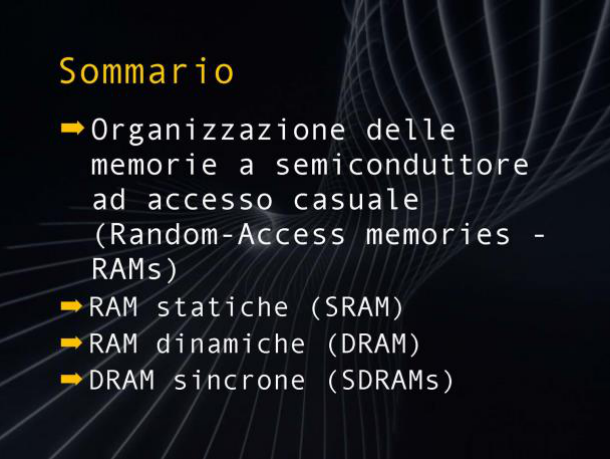
\includegraphics[width=0.40\textwidth,
                    trim=40 40 10 40, % L B R T
                    clip]
                    {images/Lez04_p01_fig_02.png}
  \caption{Sommario}
  \label{fig:Lez04_p01_fig_02}
\end{figure}
\FloatBarrier
\noindent

Ci occuperemo dell'organizzazione delle memorie a semiconduttore ad accesso casuale, chiamate anche Random Access Memories o RAMs in inglese.
Ci occuperemo delle RAM statiche, chiamate anche SRAM, delle RAM dinamiche o RAM, delle RAMs sincrone o chiamate anche SRAM.

Cominciamo con l'organizzazione delle memorie ad accesso casuale in termini generali.

\FloatBarrier
\begin{figure}[H]
  \centering
  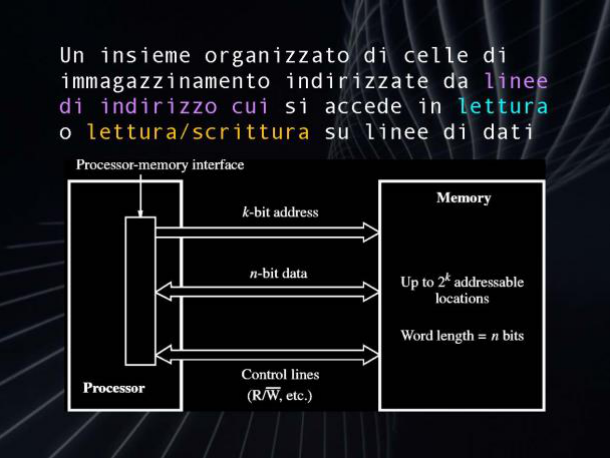
\includegraphics[width=0.60\textwidth,
                    trim=40 20 10 40, % L B R T
                    clip]
                    {images/Lez04_p01_fig_04.png}
  \caption{Sommario}
  \label{fig:Lez04_p01_fig_04}
\end{figure}
\FloatBarrier
\noindent

Questo è un insieme di celle di immagazzinamento indirizzate da linee di indirizzo a cui si accede in lettura oppure in lettura e scrittura su linee di dati.
Questo è il concetto generale di una memoria indirizzata mediante righe e colonne.
Ci sono delle righe dei segnali di indirizzo che identificano locazioni all'interno di questa memoria.
In generale vi sarà un processore che produce una richiesta.
Questa richiesta è gestita da un'interfaccia memoria-processore.

Da questa interfaccia partono k-line di indirizzo, quindi k-fili sostanzialmente, che identificano k-bit di indirizzo.
c'è un canale generalmente bidirezionale, dove sia prevista la lettura e scrittura, in cui transitano i dati.
Vi sono in fine un insieme di linee di controllo, per esempio le linee che danno il comando se si tratti di lettura read o scrittura write.
È comune questa terminologia read-write complementato per indicare che con il segnale alto è un read e con il segnale basso è un write, cioè una scrittura.
La memoria è in questo momento una scatola costituita da due alla k-locazioni indirizzabili dai questi k-bit di indirizzo.
La parola ha una lunghezza di n-bit e potrà transitare in una direzione e o nell'altra attraverso gli n-bit di i-dato.

\FloatBarrier
\begin{figure}[H]
  \centering
  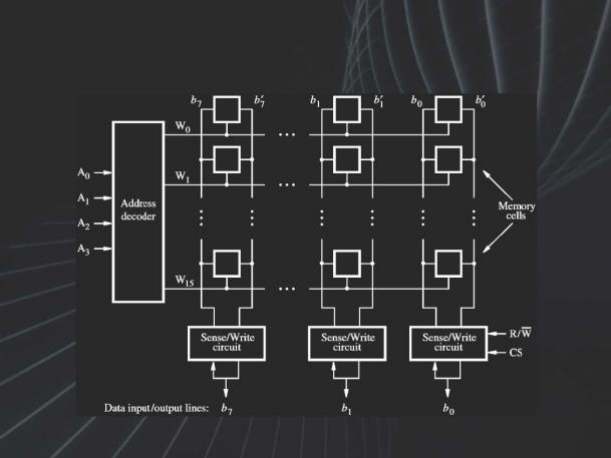
\includegraphics[width=0.80\textwidth,
                    trim=40 40 10 40, % L B R T
                    clip]
                    {images/Lez04_p01_fig_05.png}
  \caption{Semplice memoria}
  \label{fig:Lez04_p01_fig_05}
\end{figure}
\FloatBarrier
\noindent

Vediamo adesso una semplice memoria, ma che è esemplificativa, in cui abbiamo 8-bit di dato da b0 a b7, acceduti da due linee b0 negato, b1 negato, b7 negato e indirizzata da dei segnali w0 w15 che sono decodificati da un decoder a 4 ingressi e 16 uscite $2^4$.

Ognuno delle celle di locazione b0 indirizzata da w0, b0 indirizzato da w1, giù fino a b0 indirizzata da w15, ha un comune circuito di sense write, cioè di lettura e scrittura, sostanzialmente un insieme di stati di scrittura, cioè di amplificatori in scrittura e amplificatori comandati da appositi segnali read write negato e appositi segnali chip select.

All'ingresso e all'uscita di questo stadio di sense write è posto il bit 0 che proviene dalle linee di dato nel caso si tratti di una scrittura o che arriverà sulle linee di dato nel caso si tratti di una lettura notate e la freccia bidirezionale.

I segnali di read write e chip select sono applicati ugualmente a tutti i circuiti di sense write.

In questo semplice caso abbiamo 8 bit indirizzati contemporaneamente da un segnale decodificato dal decoder indirizzi. Questa è una semplice memoria 16 per 8 bit.

\FloatBarrier
\begin{figure}[H]
  \centering
  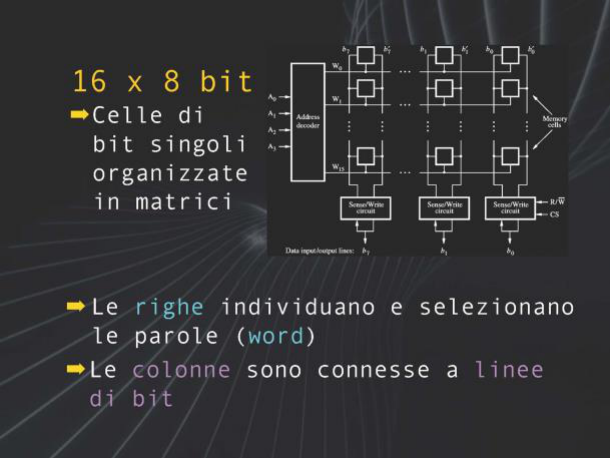
\includegraphics[width=0.60\textwidth,
                    trim=40 40 10 40, % L B R T
                    clip]
                    {images/Lez04_p01_fig_06.png}
  \caption{Memoria 16x8bit}
  \label{fig:Lez04_p01_fig_06}
\end{figure}
\FloatBarrier
\noindent

Ovviamente in questa figura abbiamo rappresentato una memoria che sia graficamente rappresentabile sullo schermo ma ovviamente potete estendere questo concetto a numeri ben più grandi come avviene nelle comuni applicazioni oggigiorno.
Le celle di bit singole sono quindi organizzate topologicamente in matrici.
Le righe individuano e selezionano le parole o word in inglese.
Le colonne sono connesse a linee di bit.
Questo è l'approccio a livello matriciale in cui tutto l'indirizzo è spezzato solo lungo una dimensione per definire ed abilitare questi elementi di memoria che al momento sono ancora delle scatole oscure.

\FloatBarrier
\begin{figure}[H]
  \centering
  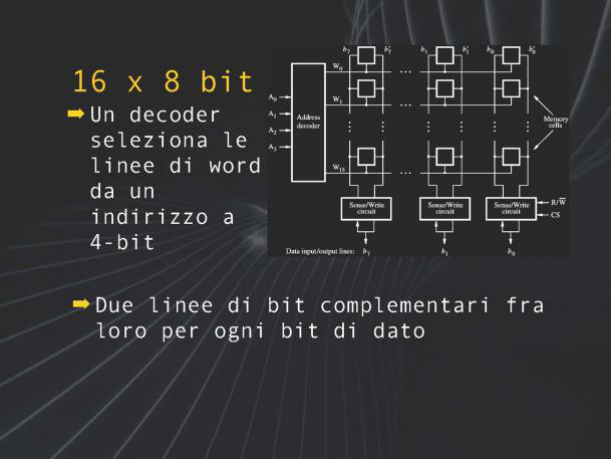
\includegraphics[width=0.60\textwidth,
                    trim=40 40 10 40, % L B R T
                    clip]
                    {images/Lez04_p02_fig_01.png}
  \caption{Memoria 16x8bit}
  \label{fig:Lez04_p02_fig_01}
\end{figure}
\FloatBarrier
\noindent

È importante osservare che il decoder che decodifica gli indirizzi che sono codificati binariamente in queste 4 linee.
2 alla 4 fa 16 quindi si va da 0 a 16 linee decodificate che selezionano gli elementi di memoria sulle 16 diverse parole.
In questo caso usiamo due linee di bit complementari fra loro per ogni bit di dato. Leveremo questo vincolo fra poco.

\FloatBarrier
\begin{figure}[H]
  \centering
  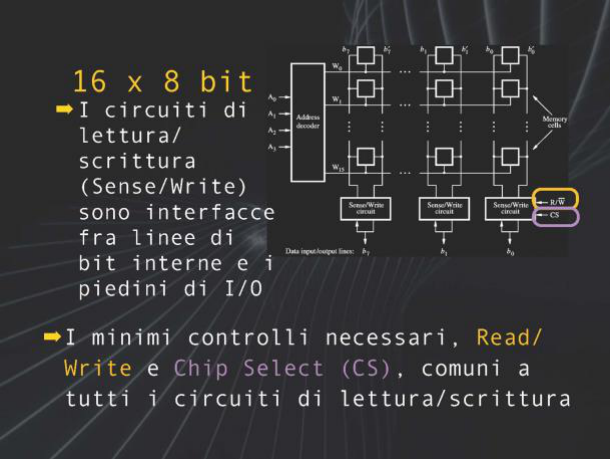
\includegraphics[width=0.60\textwidth,
                    trim=40 40 10 40, % L B R T
                    clip]
                    {images/Lez04_p02_fig_02.png}
  \caption{Memoria 16x8bit}
  \label{fig:Lez04_p02_fig_02}
\end{figure}
\FloatBarrier
\noindent


I circuiti lettura e scrittura sono delle interfacce fra le linee di bit interne e i piedini di I/O, sostanzialmente sono degli amplificatori con degli elementi che possono essere controllati in una direzione o nell'altra.
Per far funzionare questo circuito i minimi controlli necessari sono read write e chip select che abilitano o disabilitano questi chip e sono comuni a tutti i circuiti lettura e scrittura come vi ho anticipato.

\FloatBarrier
\begin{figure}[H]
  \centering
  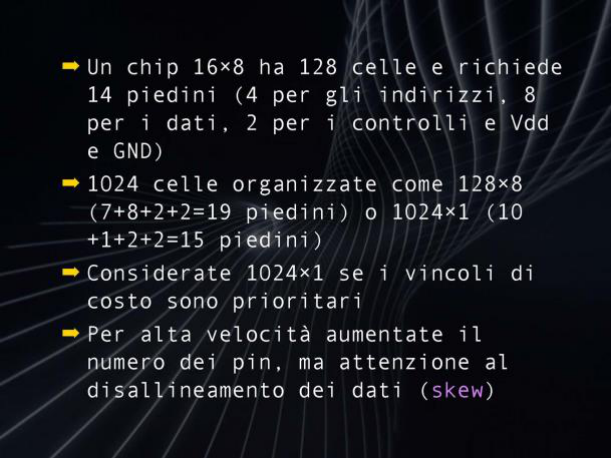
\includegraphics[width=0.60\textwidth,
                    trim=40 40 10 40, % L B R T
                    clip]
                    {images/Lez04_p02_fig_03.png}
  \caption{Memoria 16x8bit}
  \label{fig:Lez04_p02_fig_03}
\end{figure}
\FloatBarrier
\noindent

Un chip di 16x8 ha quindi 128 celle e richiede 14 piedini.
Il conteggio è semplice che ci sono 4 pin per gli indirizzi, 8 per i dati, 2 per i controlli read write e chip select e 1 per VDD e 1 per GND cioè la massa.

1024 celle possono quindi essere organizzate o come 128x8 oppure come 1024x1 con un numero di piedini in questo caso inferiore.
Il numero di piedini è pari a 10 perché 1024 è pari a $2^10$ più 1 pin di dato più 2 pin di controllo più alimentazione e massa fanno 15.
Vedete quindi che si possono fare delle scelte di progetto per definire il livello di parallelismo dei dati in uscita e questo ha un costo in termini di pin quando il parallelismo è più elevato e risparmia piedini in generale nei casi in cui non si abbiano questa esigenza.

Quindi considereremo un basso parallelismo se i vincoli di costo sui piedini sono dominanti oppure se vogliamo elevare la velocità aumenteremo il numero dei pin ma bisogna anche stare attenti al cosiddetto skew o disallineamento dei dati.
Notate infatti che questo è un problema particolarmente critico quando si aumenta la frequenza dei segnali che transitano sulle piste e le piste possono ad esempio avere diversi percorsi.

Immaginate una semplice curva che connette un piedino se avete tante piste in parallelo le piste che fanno come dire il giro corto all'interno della curva hanno un percorso inferiore alle piste che sono sul lato esterno della curva così come avviene in un normale ad esempio nella pista di atletica dove i corridori sulla pista interna se partono dalla stessa linea di partenza e arrivano alla stessa linea di partenza percorrerebbero un percorso più corto e quindi sarebbero avvantaggiati.

Questo va gestito opportunamente nei circuiti integrali dove si realizzano sistemi ad elevata velocità ne parleremo nella lezione successiva però richiamo la vostra attenzione sul fatto che aumentando il parallelismo si può aumentare la banda ma in generale bisogna aumentare maggiormente le precauzioni per evitare che i dati arrivino disallineati fra la sorgente e la destinazione.

\FloatBarrier
\begin{figure}[H]
  \centering
  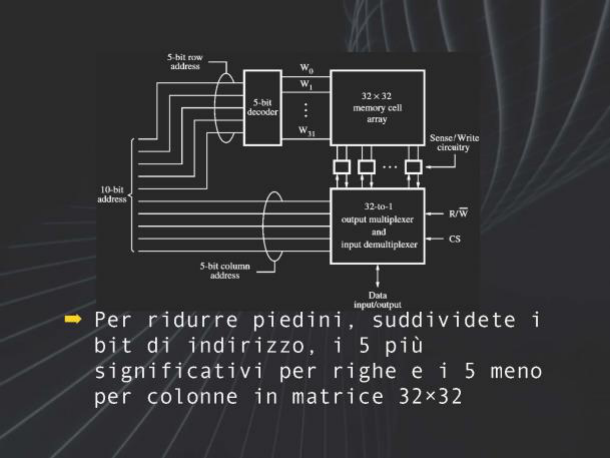
\includegraphics[width=0.80\textwidth,
                    trim=40 40 10 40, % L B R T
                    clip]
                    {images/Lez04_p02_fig_04.png}
  \caption{Riduzione numero pin}
  \label{fig:Lez04_p02_fig_04}
\end{figure}
\FloatBarrier
\noindent

Vediamo ora come si può ulteriormente ridurre il numero dei pin in un'architettura di una memoria.
Abbiamo visto che nel caso precedente semplice di un 16x8 avevamo 4 piste di indirizzo di dato.

Nel caso il numero delle piste di dato aumenti si possono partizionare le linee di dato, in questo caso vediamo 10 linee di dato, le possiamo partizionare in modo da averne 5 e 5 separate, quindi 5 andranno a costituire le cosiddette righe e 5 andranno a costituire le cosiddette colonne, non ci confondiamo con i segnali di dato, queste sono linee di indirizzo separate, quindi le più significative ad esempio sono quelle di righe e le meno significative quelle di colonna.

5 linee messe in un decoder producono 32 segnali, 5 linee messe in un multiplexer 32 in 1 decodificano questi circuiti di sense and write gli stessi che avevamo prima però ne abbiamo in questo caso 32.
Vengono multiplexati attraverso questo multiplexer 32 in 1 e 1 in 32, bilidirezionale, cioè di fatto sono due multiplexer capovolti messi l'uno contro l'altro e i dati transitano attraverso questa porta bilidirezionale ancora read write e chip select, questo cosa fa?
Permette di ridurre il numero delle piste di fatto sostanzialmente alla metà delle piste di indirizzo, quindi si suddividono i piedini di indirizzo, 5 più significativi per le righe e 5 meno significativi per le colonne e si organizza la parola in array di 32x32.
Un modulo di memoria di questo tipo può essere affiancato ad altri moduli di memoria per costruire gerarchie di memoria più elevata.

\FloatBarrier
\begin{figure}[H]
  \centering
  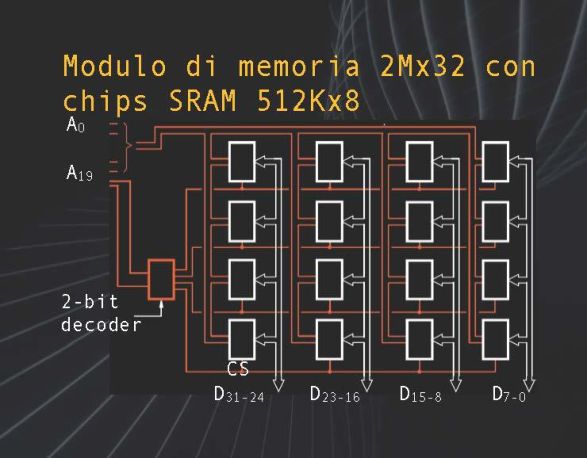
\includegraphics[width=0.80\textwidth,
                    trim=40 40 10 40, % L B R T
                    clip]
                    {images/Lez04_p02_fig_05.png}
  \caption{Memoria 2Mx32}
  \label{fig:Lez04_p02_fig_05}
\end{figure}
\FloatBarrier
\noindent

Consideriamo quindi un sistema di memoria complessivo costituito da 2 mega per 32 bit con chip sram in questo caso statici di 512k per 8 bit cada uno, vediamo quindi che per indirizzare 2 megawords servono 20 linee di dato da 0 a 19 e 2 bit per un decoder, quindi vediamo quei due di questi bit vanno a finire in un decoder, vedete un attimo quindi che i 18 piedini meno significativi vanno a indirizzare direttamente ognuno dei chip, vedete le piste sono tutte uguali e vanno a nutrire tutti questi diversi chip, i bit più significativi vengono utilizzati qua in alto per produrre i segnali di chip select ai vari chip, quindi tutti questi chip che definiscono il livello più alto, l'indirizzo più alto sono nel caso in cui i bit siano 1,1, nel caso in cui si abbia 1,0 si va su questo, in cui 0,1 si va su questa linea di 4 chip, 0,0 si va su questi qua, notate come i bit di uscita dei chip sono cablati, quindi ognuno di questi 4 chip ha i bit di dato in ingresso e in uscita cablati fra loro su delle linee comuni, qui abbiamo visto il byte di peso più significativo individuato da dato 31,24, questo è il byte meno significativo con valori da 7 a 0, quindi si indirizzano tutti i chip con gli indirizzi meno significativi, due più significativi si utilizzano per decodificarli attraverso un decoder e si pilotano i blocchi per riga, i blocchi per colonna in uscita dei pin di dato vengono fra loro cablati, questo è il modo per creare una girarchia sempre più grande, notate che non è possibile farlo in limiti arbitraria, quali sono i limiti di questa configurazione?

Innanzitutto ricordate che esistono dei limiti come il fanin e il fanout, quando andate a scrivere per esempio un dato nella memoria, il fanout dovrà essere almeno 4 in questo caso, perché vanno pilotate 1, 2, 3 e 4 porte in ingresso dalla linea che proviene qui, analogamente dovremo avere anche le linee di indirizzo che in questo caso possano pilotare niente popò di meno che 16 linee di indirizzo di ciascuno dei 16 chip utilizzati, quindi il fanout dei circuiti di pilotaggio delle linee di dato meno significativo, che peraltro sono anche quelle che più probabilmente cambiano, deve essere piuttosto potente, cioè deve essere in grado di pilotare i parassiti prevalentemente capacitivi degli ingressi di ben 16 chip, capite quindi che questa gerarchia può essere aumentata ma non indefinitivamente, alcune volte quando si aumenta il numero dei moduli, in questo caso dei chip discreti affiancati è necessario utilizzare degli stati di buffer intermedi, degli stati di tampone, buffer al fine significa questo, per separare i livelli e poter partire nuovamente.

%15:00
E' meno critica la situazione dei 2 bit più significativi che pilotano il decoder perché in questo caso il problema sarà del decoder ma ognuna delle piste del decoder deve di fatto pilotare solamente 4 chip che in questo caso corrisponde a un fanout di 4.
Dovete tenere in conto queste cose perché avere una memoria grande e una memoria veloce sono due cose che fra loro sono generalmente incompatibili e sta alla grande maestria dell'ingegnere che progetta nel cercare di ottenere il meglio dell'uno o dell'altro mondo o eventualmente un compromesso accettabile per l'applicazione fra dimensione e velocità e in continuazione si evolve, come vi ho fatto vedere in alcune delle slide delle lezioni precedenti in termini di scaling di dimensioni e di velocità.

Vi do uno spunto della riflessione e vi porto ogni volta a riflettere su quali siano i criteri per scegliere di quante righe, quante colonne e quante linee di indirizzo dotare dei chip di memoria.

\subsection{Static RAM (sRAM)}

Passiamo al prossimo argomento che è quello delle memorie statiche o static RAM.

\FloatBarrier
\begin{figure}[H]
  \centering
  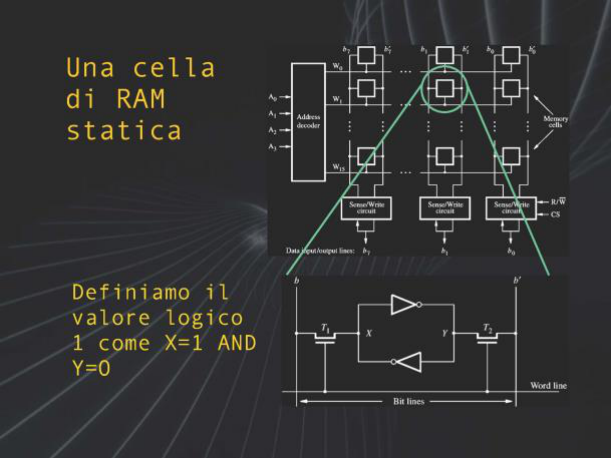
\includegraphics[width=0.80\textwidth,
                    trim=40 40 10 40, % L B R T
                    clip]
                    {images/Lez04_p03_fig_03.png}
  \caption{Static RAM}
  \label{fig:Lez04_p03_fig_03}
\end{figure}
\FloatBarrier
\noindent

Ritorniamo al nostra chip di prima in cui abbiamo detto che questo è un generico elemento di memoria e consideriamo che essa sia una cella di natura statica, quindi la generica cella è costituita da da due invertitori posti in contro in anello l'uno contro l'altro e acceduti da due pass transistor, cioè due transistori, che opportunamente aperti attraverso un segnale di tensione, quello che arriva sulla linea di parola, word line, vengono aperti e i dati che arrivano sulle linee di bit, ricordate avevamo due linee complementari, B e B', scrivono il dato contemporaneamente attraverso questi transistori.
Ovviamente deve valere che i segnali messi sulle linee B e B' siano complementari l'uno dell'altro.
Dal punto di vista pratico realizzativo questi invertitori sono realizzati in tecnologia CMOS, ma inizialmente vediamo che per esempio possiamo definire il valore logico 1 come la variabile x, lo stato interno uguale a 1, e dal punto di vista strettamente logico la variabile y uguale a 0.
Lo stato logico 0 di questa cella sarà quindi scambiando i valori di x e y.

\FloatBarrier
\begin{figure}[H]
  \centering
  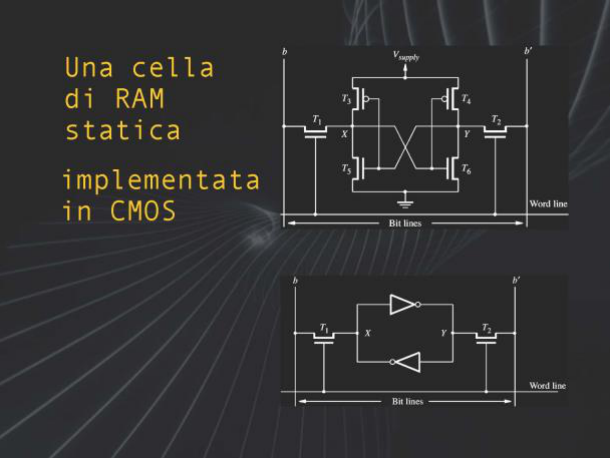
\includegraphics[width=0.80\textwidth,
                    trim=40 40 10 40, % L B R T
                    clip]
                    {images/Lez04_p03_fig_04.png}
  \caption{Riduzione numero pin}
  \label{fig:Lez04_p02_fig_04}
\end{figure}
\FloatBarrier
\noindent

Quindi la implementiamo in CMOS e per implementare CMOS i due invertitori non sono altro che i classici invertitori CMOS connesse le uscite con gli ingressi, e questo corrisponde esattamente alla rappresentazione dal punto di vista logico di questi due buffer invertitori, stati invertitori.

Vi invito a riflettere quali siano le principali problematiche delle SRAM.
Vi chiedo se possiamo usarle sempre.

\subsection{RAM dinamiche}

Prossimo argomento che è quello delle RAM dinamiche.

\FloatBarrier
\begin{figure}[H]
  \centering
  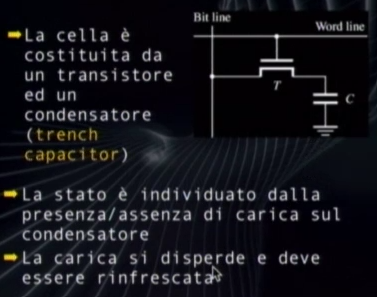
\includegraphics[width=0.70\textwidth,
                    trim=0 0 0 0, % L B R T
                    clip]
                    {images/Lez04_p03_fig_06a.png}
  \caption{Riduzione numero pin}
  \label{fig:Lez04_p03_fig_06a}
\end{figure}
\FloatBarrier
\noindent

La cella di una RAM dinamica è costituita da un transistore ed un solo condensatore, questo condensatore è chiamato trench capacitors.
Quindi in questo caso c'è una wordline, una bitline, un transistor, un pass-transistor che abilita un percorso a bassa impedenza verso un condensatore quando la wordline è selezionata oppure stabilisce un livello di alta impedenza e quindi isola la carica che è immagazzinata su questo condensatore.
Lo stato logico è individuato dalla presenza o assenza di carica sul condensatore.
Ovviamente presenza e assenza sono definite rispetto a una qualche soglia che discrimina un livello alto da un livello basso di tensione, quindi dalla presenza di una carica o dall'assenza di una carica.
Dal punto di vista la carica si disperde e quindi deve essere rinfrescata di tanto in tanto.
Questo è uno dei punti più critici delle DRAM perché mentre l'invertitore CMOS nella cella SRAM che avevamo visto prima, fintanto che l'alimentazione rimane, lo stato rimane tal quale non è modificato a prescindere dalla lettura, in questo caso vedremo che lo stato decade sia quando viene letto che a prescindere dalla lettura semplicemente perché il transistorio ha delle perdite, o  per la stessa realizzazione del condensatore che ha delle perdite.
Vi do una rappresentazione un po' schematica ma abbastanza importante di come è fatto questo transistore dal punto di vista fisico.

\FloatBarrier
\begin{figure}[H]
  \centering
  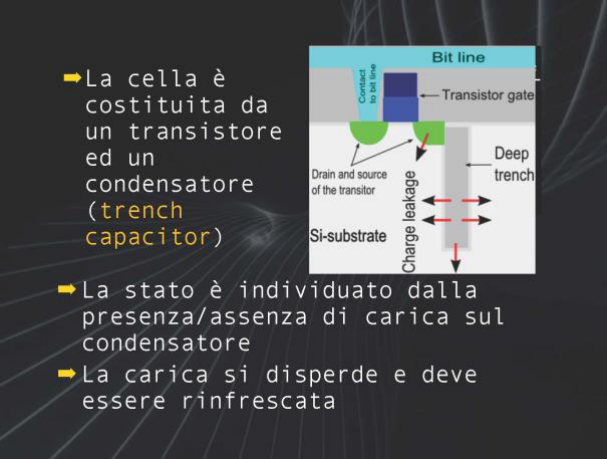
\includegraphics[width=0.70\textwidth,
                    trim=40 40 40 40, % L B R T
                    clip]
                    {images/Lez04_p04_fig_01.png}
  \caption{Riduzione numero pin}
  \label{fig:Lez04_p04_fig_ì1}
\end{figure}
\FloatBarrier
\noindent

Qua vediamo una bit line che è una pista metallizzata che contatta il drain cioè il collettore di un transistore MOS, qui c'è il gate o porta del transistore, questo è l'ossido di gate, qui c'è il source o sorgente del transistore che connette attraverso questa struttura che in inglese si chiama recess cioè scavata profondamente, è un deep trench, una profonda trincea, letteralmente significa profonda trincea in cui è stato scavato un buco nel silicio, nel substrato di silicio, è stato depositato un conduttore attorno al buco, è stato depositato uno strato di dielectrico, diciamo un ossido per esempio dell'ossio silicio anche se ormai non è più soltanto ossio silicio e sopra è stata applicata un'ulteriore metallizzazione per realizzare il secondo piatto del condensatore, questa struttura è connessa a massa attraverso l'elettrodo, diciamo attraverso la superficie esterna del condensatore ed è connesso al source del transistore attraverso l'elettrodo depositato sopra, quindi notate che ovviamente la struttura non è perfettamente in scala però rappresenta un po' il principio, per guadagnare in superficie e quindi in capacità del transistore è necessario realizzare un buco profondo per aumentare la superficie complessiva, questo è un processo che rende il processo leggermente diverso rispetto al normale processo CMOS e quindi le memorie DRAM vengono realizzate su linee generalmente non perfettamente standard rispetto a quelle dei comuni processori, cioè che realizzano CMOS, su questo torneremo più avanti quando parleremo di un particolare tipo di cache, le cosiddette embedded DRAM, in questo momento è importante per voi sapere che generalmente questa tecnologia non è pienamente compatibile con quella con cui si realizzano i microprocessori.

La cella è molto semplice, qui c'è una sola cella di porta mentre ne avevamo due nella SRAM, c'è un solo condensatore di memoria mentre ne avevamo quattro, due CMOS controreazionati nel caso della SRAM.

\FloatBarrier
\begin{figure}[H]
  \centering
  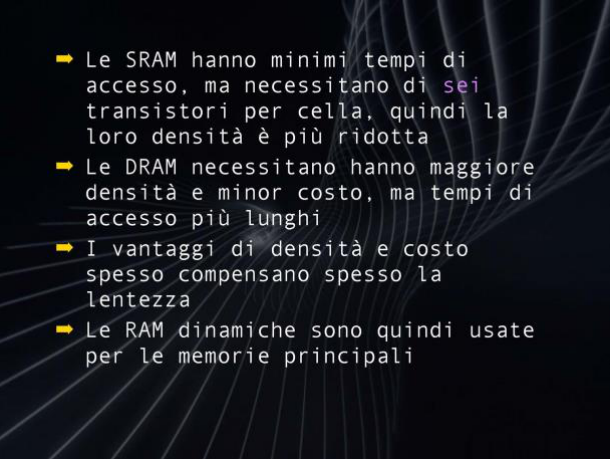
\includegraphics[width=0.70\textwidth,
                    trim=0 0 0 0, % L B R T
                    clip]
                    {images/Lez04_p04_fig_02.png}
  \caption{Confronto SRAM-DRAM}
  \label{fig:Lez04_p04_fig_02}
\end{figure}
\FloatBarrier
\noindent



Ripetiamo il concetto, 

le SRAM hanno minimi tempi di accesso perché il dato è già scritto ma necessitano di ben sei transistori per cella, quindi la densità è più ridotta di quanto non sia possibile ottenere con le DRAM che possono avere una maggiore densità e minor costo, perché il costo è legato sostanzialmente al numero dei passi e alla densità degli elementi che si trovano per unità di area ma hanno generalmente i tempi di accesso più lunghi perché è necessario leggere la scarica esponenziale del condensatore attraverso i circuiti di SENSE e al contrario delle SRAM che si comportano sostanzialmente come dei generatori di tensione, cioè l'uscita diretta degli stadi CMOS.

Analogamente la scrittura è fatta attraverso la carica di un condensatore che anche questa avviene con un andamento esponenziale, quindi sostanzialmente la natura intrinseca della scarica e della carica di un condensatore determina dei tempi di lettura e scrittura più lunghi.

Però in generale i vantaggi di densità e costo delle DRAM compensano quasi sempre, spesso almeno, la lentezza intrinseca del processo e quindi le RAM dinamiche sono utilizzate per le memorie principali delle architetture di elaborazione in quasi tutti i casi, salvo in quei casi tipo piccoli microcontrollori a basso consumo, dove si preferisce utilizzare ancora delle SRAM perché in condizioni diciamo normali, senza commutazione, non sono soggetti a significative perdite di potenza. Al contrario le DRAM devono essere rinfrescate e quindi intrinseicamente dissipano.
%25:01
\FloatBarrier
\begin{figure}[H]
  \centering
  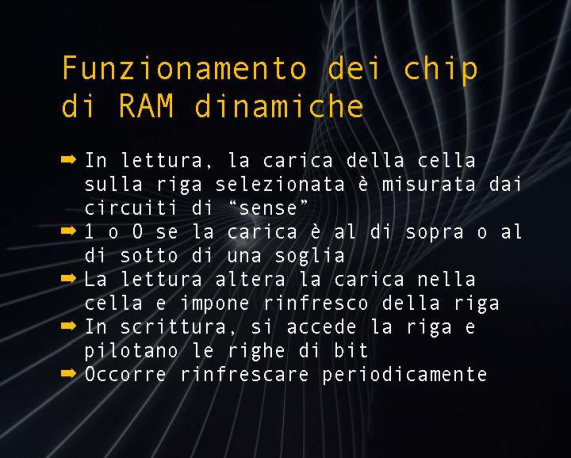
\includegraphics[width=0.70\textwidth,
                    trim=50 60 40 50, % L B R T
                    clip]
                    {images/Lez04_p04_fig_03.png}
  \caption{RAM dinamiche}
  \label{fig:Lez04_p04_fig_03}
\end{figure}
\FloatBarrier
\noindent

Vediamo quindi il funzionamento dei chip di RAM dinamiche.
In lettura la carica della cella sulla riga selezionata è misurata dai circuiti di sense, cioè leggendo la capacità, 1 o 0 se la carica è al di sopra o al di sotto di una soglia.
La lettura stessa altera la carica della cella e quindi impone il rinfresco della riga, quindi è necessario leggere la riga e prendere il valore e riscriverlo nuovamente attraverso la linea di bit, in questo caso una sola linea di bit.
In scrittura si accede alla riga e si pilotano le righe di bit, diciamo di tutta la parola.
Anche questa scrittura viene coi tempi caratteristici della carica di un condensatore, cioè comune esponenziale.
Occorre rinfrescare periodicamente anche se nulla viene letto, perché, come vi ho detto, vi è una intrinseca dissipazione attraverso il dielectrico del condensatore e attraverso, eventualmente anche se in piccola quantità attraverso la porta del transistor che abilita il condensatore.

\FloatBarrier
\begin{figure}[H]
  \centering
  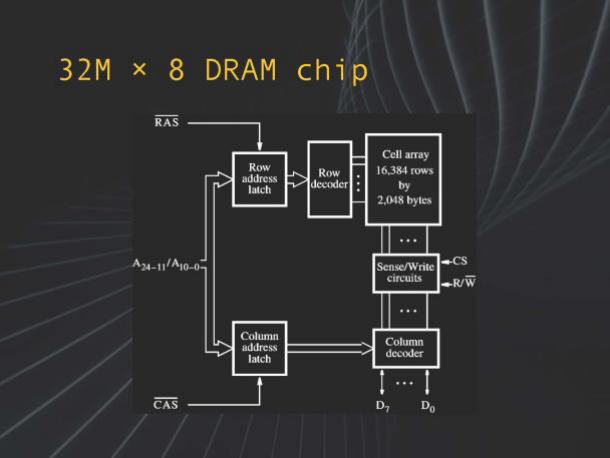
\includegraphics[width=0.70\textwidth,
                    trim=50 30 90 50, % L B R T
                    clip]
                    {images/Lez04_p04_fig_04.png}
  \caption{RAM dinamiche}
  \label{fig:Lez04_p04_fig_04}
\end{figure}
\FloatBarrier
\noindent

Vediamo quindi come è realizzata una DRAM, in questo caso 32 Mega per 8, questo chip.
In questo caso c'è un row address latch, un column address latch, cioè un latch che memorizza temporaneamente la parte di riga e la parte di colonne, gli indirizzi sono separati fra riga e colonne, si utilizzano due segnali che saranno fondamentali per chiunque pensa di guardare una memoria, i cosiddetti RAS e CAS, row address strobe e column address strobe ancora attivi bassi, vi è un decoder degli indirizzi di riga che seleziona la cella, analogamente un decoder di colonna, in questo caso avevamo un multiplexer, in questo caso utilizziamo un decoder, ma vedete che non cambia molto nella questione, e ancora nuovamente i circuiti di sense e write, la nostra cella costituita di 16.384 righe per 2.048 colonne, cioè 11 linee di bit per le colonne e 14 per le righe, quindi il progettista ha preferito utilizzare 14 linee di riga e 11 di colonna.

\FloatBarrier
\begin{figure}[H]
  \centering
  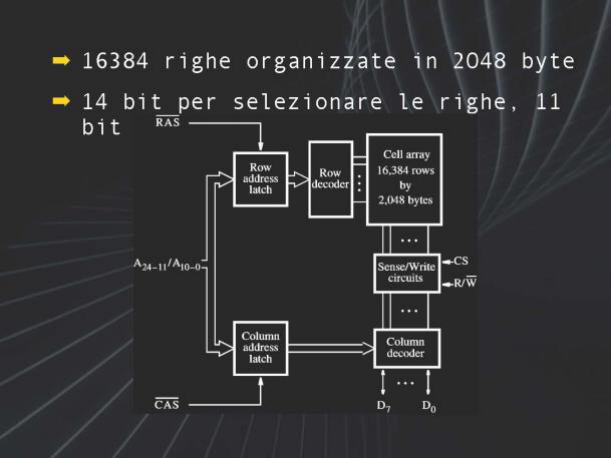
\includegraphics[width=0.70\textwidth,
                    trim=40 30 20 40, % L B R T
                    clip]
                    {images/Lez04_p04_fig_05.png}
  \caption{RAM dinamiche}
  \label{fig:Lez04_p04_fig_05}
\end{figure}
\FloatBarrier
\noindent

\FloatBarrier
\begin{figure}[H]
  \centering
  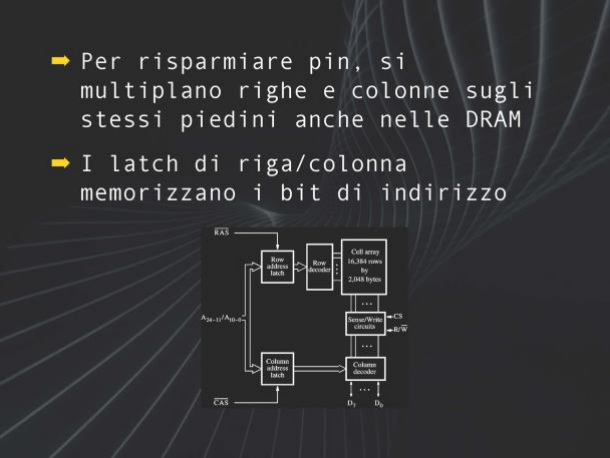
\includegraphics[width=0.70\textwidth,
                    trim=40 30 20 40, % L B R T
                    clip]
                    {images/Lez04_p04_fig_06.png}
  \caption{RAM dinamiche}
  \label{fig:Lez04_p04_fig_06}
\end{figure}
\FloatBarrier
\noindent

Per risparmiare i pin è possibile multiplare le righe e le colonne sugli stessi i piedini, anche nelle DRAM, e questo è quello che tipicamente avviene, perché i piedini sono importanti, perché determinano il costo del circuito.
I latch di riga e colonna memorizzano i bit di indirizzo per tenere gli indirizzi più stabili.

\FloatBarrier
\begin{figure}[H]
  \centering
  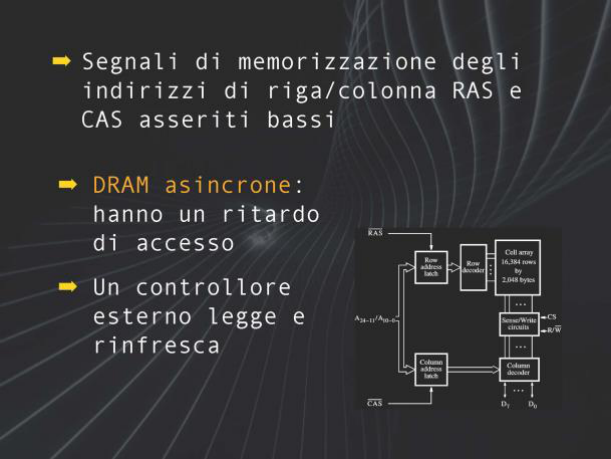
\includegraphics[width=0.70\textwidth,
                    trim=40 30 20 40, % L B R T
                    clip]
                    {images/Lez04_p05_fig_01.png}
  \caption{RAM dinamiche}
  \label{fig:Lez04_p05_fig_01}
\end{figure}
\FloatBarrier
\noindent

I segnali di memorizzazione degli indirizzi di riga e di colonna sono asseriti bassi, notate che la multiplazione di indirizzi di riga e di colonna di fatto impone l'esistenza di almeno un latch, in questo caso ne utilizziamo due, perché prima scriviamo l'indirizzo di riga, poi selezioniamo l'indirizzo di colonna, è chiaro che l'indirizzo di riga deve essere in qualche modo memorizzato.
Queste sono le cosiddette DRAM asincrone, hanno un ritardo di accesso legato ai tempi di scrittura delle righe e di colonne, un controllore esterno legge e periodicamente rinfresca tutte le memorie, sono state le prime DRAM ad essere utilizzate.

\FloatBarrier
\begin{figure}[H]
  \centering
  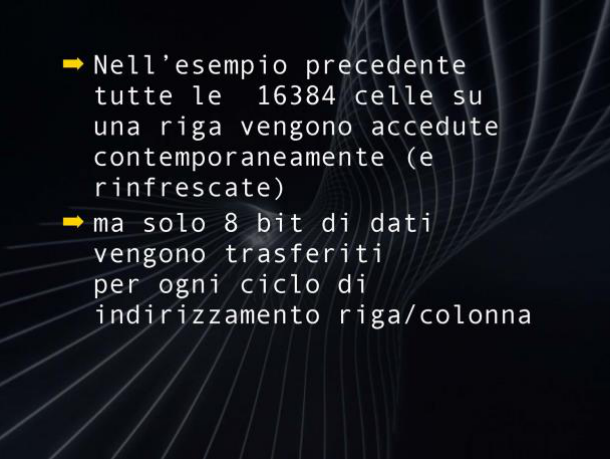
\includegraphics[width=0.70\textwidth,
                    trim=40 30 20 40, % L B R T
                    clip]
                    {images/Lez04_p05_fig_02.png}
  \caption{RAM dinamiche}
  \label{fig:Lez04_p05_fig_02}
\end{figure}
\FloatBarrier
\noindent

Nell'esempio precedente tutte le 16.384 celle su una riga vengono accedute contemporaneamente e rinfrescate periodicamente perché il dato venga mantenuto.
Notate che però solo 8 bit di dati vengono trasferiti per ogni ciclo di indirizzamento e di riga, quindi ogni volta bisogna applicare un RAS e un CAS per prendere una semplice parola di 8 bit di dato.
Notate che quindi sono necessarie due operazioni di scrittura sul basso indirizzo per accedere a un dato in lettura o scrivere il dato in fase di scrittura.
Vi accorgete che questo ha chiaramente dei costi in termini di tempo e vi do quindi il solito spunto per la riflessione e vi invito a pensare come si potrebbe incrementare la velocità rispetto al funzionamento asincrono.

\subsection{RAM Sincrone (SDRAM)}

Passiamo quindi ad affrontare l'argomento delle RAM sincrone o Synchronous Dynamic RAMs RAM in inglese.

\FloatBarrier
\begin{figure}[H]
  \centering
  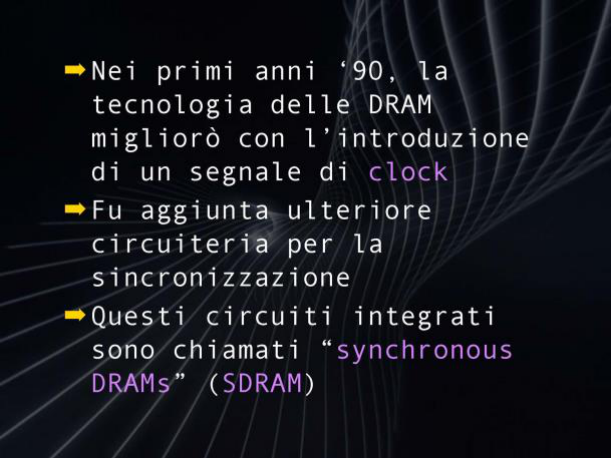
\includegraphics[width=0.70\textwidth,
                    trim=40 30 20 40, % L B R T
                    clip]
                    {images/Lez04_p05_fig_05.png}
  \caption{RAM dinamiche}
  \label{fig:Lez04_p05_fig_05}
\end{figure}
\FloatBarrier
\noindent

Nei primi anni 90 la tecnologia delle DRAM migliorò con l'introduzione di un segnale di clock all'ingresso delle DRAM.
Fu aggiunta ulteriore circuiteria per la sincronizzazione e questi circuiti integrati così sincronizzati da un clock sono chiamati Synchronous DRAM o SDRAM.
Vediamo come è costituita questa DRAM diciamo nella configurazione semplice.

\FloatBarrier
\begin{figure}[H]
  \centering
  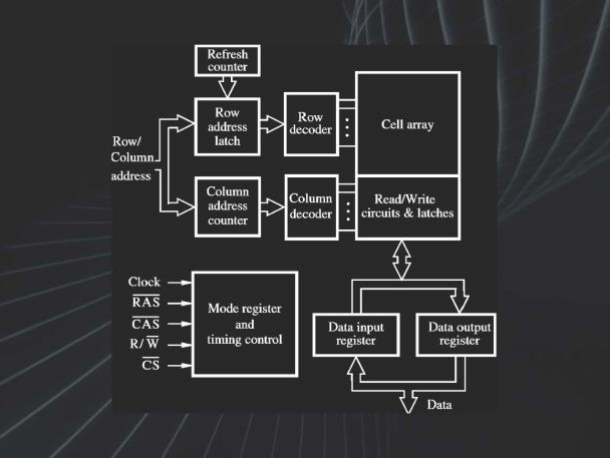
\includegraphics[width=0.80\textwidth,
                    trim=40 30 20 40, % L B R T
                    clip]
                    {images/Lez04_p05_fig_06.png}
  \caption{RAM dinamiche}
  \label{fig:Lez04_p05_fig_06}
\end{figure}
\FloatBarrier
\noindent

Ancora abbiamo il raw address latch perché le righe e le colonne sono multiplexate e l'abilitazione è sempre determinata da RAS e CAS, in aggiunta al raw address latch, cioè al latch dell'indirizzo di riga, si mette un contatore di rinfresco che va a scandire quindi gli indirizzi. Quindi questo è un contatore aggiuntivo.

C'è un ulteriore contatore di colonne e poi a valle di questi vi sono dei decoder. Qui c'è la cella di array e quindi qui ancora i vari circuiti di read write, sense e dei latch.

La cosa interessante è che in uscita non vi è l'uscita direttamente attraverso un decoder o un multiplexer come abbiamo visto precedentemente, ma vi sono dei registri sincroni rispetto al clock.
Qui è un data input register, cioè un registro in fase di ingresso e un registro in fase di uscita.
Una sequenza di circuterie aggiuntive che producono i sincronismi per tutto questo circuito clock, RAS e CAS negati, read write e chip select.
Quindi il sistema aumenta in termini di variabili in ingresso perché c'è anche il clock e soprattutto aumenta perché vi sono due registri dei dati e due contatori per definire gli indirizzi che non vengono più mandati semplicemente ma vengono anche aggiornati internamente.

\FloatBarrier
\begin{figure}[H]
  \centering
  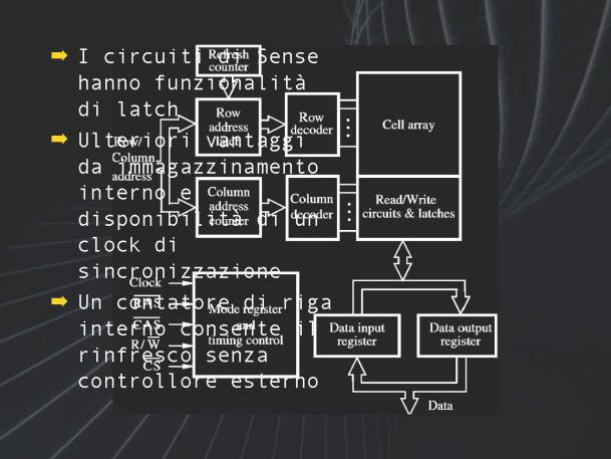
\includegraphics[width=0.80\textwidth,
                    trim=0 0 0 0, % L B R T
                    clip]
                    {images/Lez04_p06_fig_01.png}
  \caption{RAM dinamiche}
  \label{fig:Lez04_p06_fig_01}
\end{figure}
\FloatBarrier
\noindent


In questo caso i circuiti di sense hanno una funzione di latching del dato e ulteriori vantaggi da immagazzinamento interno e disponibilità di clock e di sincronizzazione permettono di aumentare il flusso dei dati, la velocità del flusso dei dati.
Il contatore di riga interno consente il rinfresco delle celle di memoria indipendentemente da un controllore esterno.
Come avevo detto nelle DRAM asincrone era necessario produrre da un controllore esterno la sequenza con RAS e CAS per rinfrescare tutta la celle.
In questo caso deve solo arrivare un comando di rinfresco, il refresh counter fa la scansione degli indirizzi di riga e quindi vengono riscritti, si fa la scansione della celle e analogamente il contatore di indirizzi di colonna fa il rinfresco.

E quindi è anche possibile fare il rinfresco senza dover mandare in continuazione dall'esterno i segnali di riga e colonna RAS e CAS.
Notate che questo oltre ad avere una semplificazione per il controllore della memoria esterna, riduce anche il consumo di potenza perché non è più necessario scrivere ripetutamente gli indirizzi di riga e di colonna e asserire RAS e CAS attraverso magari delle piste lunghe diverse centimetri, quindi dotate di una capacità e per ogni capacità c'è un $1/2*C*V^2$ di energia dissipata per ogni commutazione.
In questo caso viene tutto realizzato internamente e quindi può procedere più rapidamente oppure semplicemente dissipare meno.
In generale sono vere entrambe le cose, cioè si dissipa meno e si può realizzare il rinfresco in maniera più rapida.
E' importante che l'esistenza dei contatori di colonna permettono di scandire la riga senza dover riasserire nuovamente il segnale di row address strobe per indirizzi contigui sulla stessa riga.
Questo permette il trasferimento di più parole aventi la stessa riga di indirizzo ma colonne consecutive.
Questo fa sì che non sia necessario riasserire ripetutamente RAS.

\FloatBarrier
\begin{figure}[H]
  \centering
  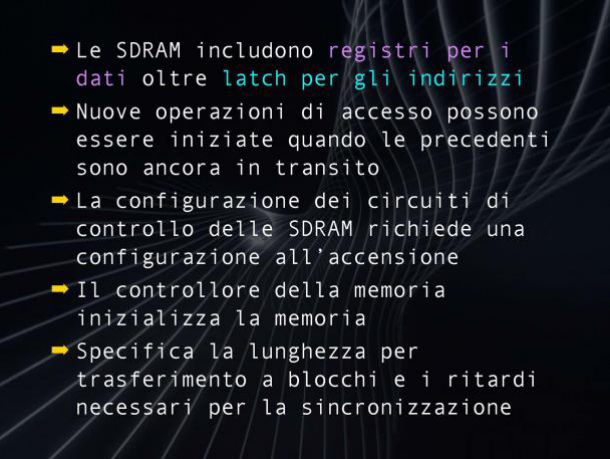
\includegraphics[width=0.80\textwidth,
                    trim=30 30 30 30, % L B R T
                    clip]
                    {images/Lez04_p06_fig_02.png}
  \caption{RAM dinamiche}
  \label{fig:Lez04_p06_fig_02}
\end{figure}
\FloatBarrier
\noindent

Vediamo quindi che le SDRAM includono registi di dati oltre che latch per gli indirizzi.
Le nuove operazioni di accesso possono essere iniziate quando le precedenti sono ancora in transito grazie ai registi di ingresso e di uscita dei dati.
Le configurazioni dei circuiti di controllo delle SDRAM, la configurazione richiede una configurazione all'accensione, cioè la SDRAM deve essere educata sul da farsi.
Il controllore della memoria inizializza semplicemente la memoria ma non deve più nuovamente rinfrescarla come avviene nelle DRAM asincrone.
Il controllore specifica inoltre, la lunghezza per il trasferimento a blocchi e i ritardi necessari per la sincronizzazione.

\FloatBarrier
\begin{figure}[H]
  \centering
  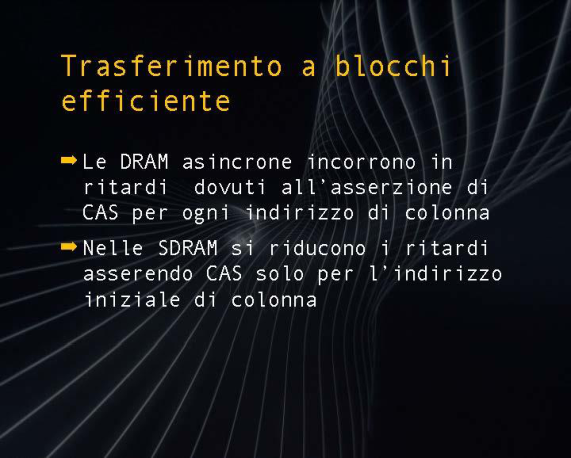
\includegraphics[width=0.80\textwidth,
                    trim=40 120 40 30, % L B R T
                    clip]
                    {images/Lez04_p06_fig_03.png}
  \caption{RAM dinamiche}
  \label{fig:Lez04_p06_fig_03}
\end{figure}
\FloatBarrier
\noindent

Questo consente di ottenere trasferimenti a blocchi efficienti.
Le DRAM asincrone incorrono infatti i ritardi dovuti all'assersione di RAS e CAS per ogni indirizzo di colonna.
Mentre nelle SDRAM si riducono i ritardi asserendo colon address strobe solo per l'indirizzo iniziale di colonna e poi il contatore interno dei registi di colonna aggiorna gli indirizi e decodifica elementi sulla stessa riga di indirizzo ma con colonne consecutive.

\FloatBarrier
\begin{figure}[H]
  \centering
  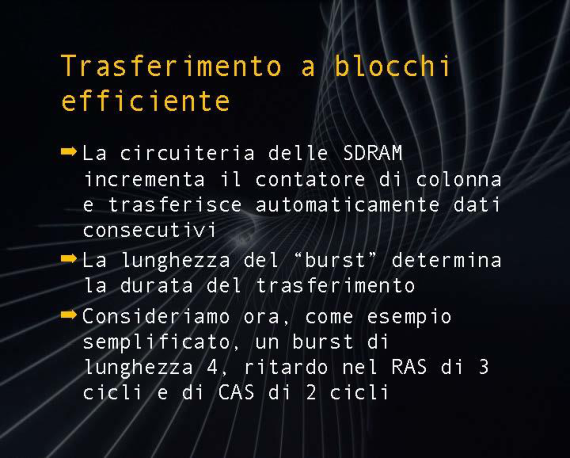
\includegraphics[width=0.80\textwidth,
                    trim=40 40 40 30, % L B R T
                    clip]
                    {images/Lez04_p06_fig_04.png}
  \caption{RAM dinamiche}
  \label{fig:Lez04_p06_fig_04}
\end{figure}
\FloatBarrier
\noindent

Il trasferimento a blocchi, abbiamo detto, è efficiente perché la circuteria delle SDRAM incrementa il contatore di colonna e trasferisce automaticamente dati consecutivi.
La lunghezza del burst determina la lunghezza del trasferimento.
burst è un evento improvviso e veloce.
Consideriamo ora, come esempio semplificato, un burst di lunghezza 4, ritardo nel RAS di 3 cicli e di CAS nei 2 cicli.
Questo è un esempio molto semplificativo ma ci permette di rappresentarlo graficamente sullo schermo.
Nella realtà i ritardi sono sensibilmente più lunghi ma è utile dal punto di vista didattico.

\FloatBarrier
\begin{figure}[H]
  \centering
  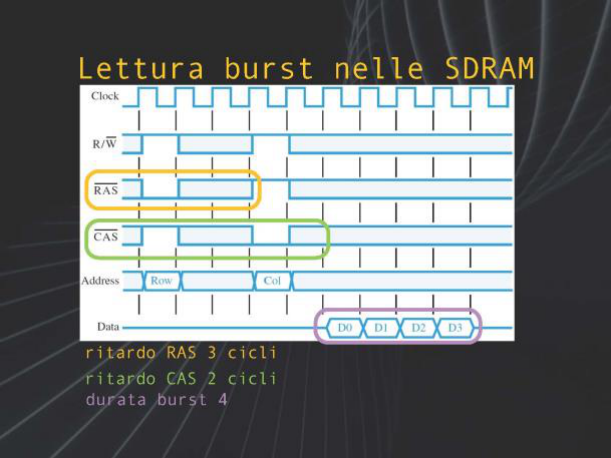
\includegraphics[width=0.80\textwidth,
                    trim=40 40 40 30, % L B R T
                    clip]
                    {images/Lez04_p06_fig_05.png}
  \caption{RAM dinamiche}
  \label{fig:Lez04_p06_fig_05}
\end{figure}
\FloatBarrier
\noindent

Guardiamo quindi l'oscillogramma della nostra memoria in cui abbiamo un clock, i segnali di read-write, RAS e CAS negati, le linee di indirizzo e le linee di dati.
Questa terminologia ci dice che qui vengono messi gli indirizzi di riga, qui vengono messi gli indirizzi di colonna rispetto al clock, qui vengono prodotti i dati, quindi il resto dei dati.
Il segnale read-write alto, alto sta per read, il segnale RAS e CAS sono asseriti bassi, notate che RAS è asserito prima perché prima si mandano gli indirizzi di riga, vedete il ritardo tra RAS e CAS è di tre cicli perché il tempo che RAS è asserito non si può assedire CAS prima che partano almeno tre cicli.
Dopo che è asserito CAS con due cicli di latenza, compaiono i dati, quindi vedete che dopo l'assersione di CAS, le linee di dati sono asserite.
Dopo due cicli sono disponibili i dati, questo è un esempio molto semplificativo, altrimenti avremmo avuto questo grafico molto più largo e meno visibile, infine abbiamo deciso che il nostro burst è costituito di quattro dati che vengono tirati fuori sincroni sul fronte positivo del clock e quindi raccolti.
Notate che se avessimo dovuto riasserire RAS e CAS per ognuno di questi dati, chiaramente i tempi sarebbero stati sensibilmente più lunghi.

Vi invito a fare il calcolo del vantaggio temporale avendo mantenuto le stesse tempistiche di RAS e CAS, quindi tre cicli per RAS e due di CAS, quanti cicli complessivi servirebbero nel caso in cui la memoria sia completamente asincrona invece che sincrona come la presente.

Con questo vi do uno spunto per la riflessione e vi chiedo come si potrebbe ulteriormente incrementare la velocità rispetto al funzionamento sincrono sul fronte del clock.
% ------------------------------------------------------------


% ------------------------------------------------------------
% ESEMPIO FIGURA PERFETTAMENTE GESTITA
% ------------------------------------------------------------
% \FloatBarrier
% \begin{figure}[H]
%   \centering
%   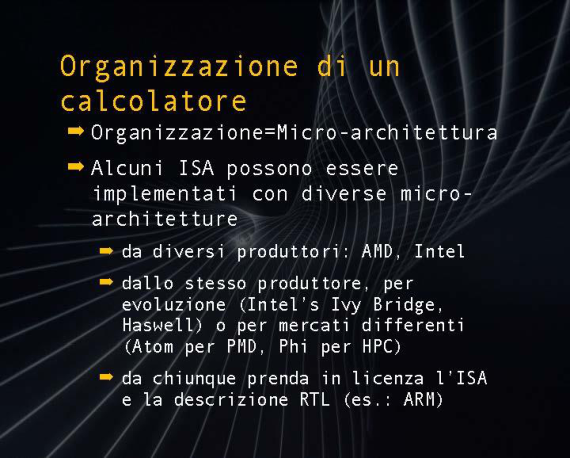
\includegraphics[width=0.6\textwidth, trim=40 40 15 40, clip]{images/Lez02_p04_fig_04.png}
%   \caption{Approccio olistico}
%   \label{fig:Lez02_p04_fig_04}
% \end{figure}
% \FloatBarrier
% \noindent
% Testo che segue immediatamente la figura senza spazi indesiderati.
% ------------------------------------------------------------

\end{document}
